% --- Chapitre 4 : Partie Distribution ---
\chapter{Distribution}

    \section{Rice Cooker}

Rappel des valeurs obtenues lors du rapport 1~:

Dans ce second rapport nous allons, à l'aide des valeurs trouvées dans le premier rapport, détailler la conception du convertisseur DC/DC permettant d'adapter le rice-cooker à notre réseau continu. Afin de garantir un fonctionnement transparent pour l'utilisateur tout en protégeant le parc de batteries, la puissance a été bridée à 450~W.
La caractérisation préalable de la charge (quasi-résistive, $R = 78~\Omega$) a permis de figer les contraintes électriques strictes que devra respecter notre hacheur élévateur~:

\begin{itemize}
    \item \textbf{Entrée (Batteries)}~: Tension $V_e = 50~\text{V}$, appelant un courant d'entrée moyen $I_e = 9~\text{A}$.
    \item \textbf{Sortie (Charge)}~: Tension $V_S = 187,5~\text{V}$ délivrant un courant $I_S = 2,40~\text{A}$.
    \item \textbf{Gain statique exigé}~: $G = 3,75$.
\end{itemize}

Pour répondre à ces différentes caractéristiques, nous avons étudié deux convertisseurs différents puis simulé avec PSIM afin de comparer les différents avantages et inconvénients de ces montages.

        \subsection{Solutions techniques}

\subsubsection*{Différentes topologies de convertisseurs}

\textbf{Hacheur dual boost entrelacé~:}

C'est une structure composée de deux hacheurs boost classiques qui sont entrelacés. L'avantage de celui-ci étant que l'on va répartir le temps de fonctionnement sur 2 mailles différentes, ce qui va permettre de réduire l'ondulation de courant puisqu'elle sera répartie sur 2 inductances identiques. 

\begin{figure}[H]
    \centering
    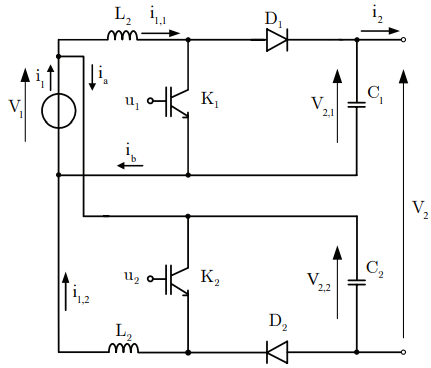
\includegraphics[width=0.8\linewidth]{images/Partie Rice cooker/01_Schéma hacheur entrelacé.png}
    \caption{Schéma Hacheur dual boost entrelacé.}
\end{figure}

Pour dimensionner les composants de ce hacheur, on utilise la même méthode que pour un hacheur boost classique car il s'agit simplement de deux hacheurs boost classiques entrelacés.

En connaissant nos valeurs de tensions d'entrée et de sortie et de courants d'entrée et de sortie, on peut dimensionner un hacheur boost qui conviendrait pour~:

\begin{tracebox}[Dimensionnement Hacheur Dual Boost Entrelacé]
\textbf{Hypothèses :} Conduction continue, ondulation de courant de $100\%$ ($\Delta i_L = I_L$) et ondulations de tension admissibles ($\Delta V_e = 10 \, \text{V}$, $\Delta V_s = 20 \, \text{V}$). Fréquence $F = 100 \, \text{kHz}$. \\
\textbf{Formules :} 
$$ \alpha_{\text{nom}} = \frac{V_S - V_e}{V_S + V_e} \quad ; \quad L = \frac{\alpha \cdot V_e}{\Delta i_L \cdot F} $$
\textbf{Application numérique :} 
$$ \alpha_{\text{nom}} = \frac{188 - 50}{188 + 50} = 0.58 $$
$$ I_L = \frac{I_s}{1-\alpha} = \frac{2.39}{0.266} \approx 9 \, \text{A} $$
$$ L = \frac{0.734 \cdot 50}{9 \cdot 10^5} = 41 \, \mu\text{H} \quad \text{(avec } \alpha=0.734 \text{ dans l'équation boost pur)} $$
\end{tracebox}

En choisissant une ondulation en tension de 10~V pour l'entrée et 20~V pour la sortie, on obtient des valeurs de condensateurs pour l'entrée et la sortie. On peut prendre une ondulation de tension assez conséquente car le but de notre convertisseur va être d'alimenter un appareil qui va juste chauffer des aliments par effet Joule, donc c'est surtout la valeur moyenne qui nous importe.

$$ C_e = \frac{\Delta i_L}{8 \cdot F \cdot \Delta V_e} = \frac{9}{8 \cdot 10^5 \cdot 10} \approx 1~\mu\text{F} $$

$$ C_s = \frac{I_s \cdot \alpha \cdot T}{F \cdot \Delta V_s} = \frac{2,39 \cdot 0,734}{10^5 \cdot 20} \approx 1~\mu\text{F} $$

Le principal problème qui va se poser avec le hacheur boost classique est le rapport cyclique relativement élevé du signal PWM pour commander le transistor. En effet, lorsque le rapport cyclique devient trop élevé, on a une différence croissante entre les performances théoriques et les performances réelles de notre convertisseur qui sont largement diminuées.

Le hacheur dual boost entrelacé fonctionne avec un rapport cyclique nettement moins élevé (0,580 contre 0,734 pour le boost classique). De plus, c'est la solution la plus efficace que l'on pourrait retenir car l'on réduit l'ondulation de courant dans les inductances puisque le stockage est réparti dans deux inductances séparées. Cependant, cette structure possède beaucoup de composants donc elle est plus chère et elle nécessite absolument une commande isolée car le point de référence de la source d'un des deux transistors n'est pas à la masse. C'est la meilleure solution mais aussi la plus complexe à mettre en œuvre.

\textbf{Hacheur dual boost en T~:}

\begin{figure}[H]
    \centering
    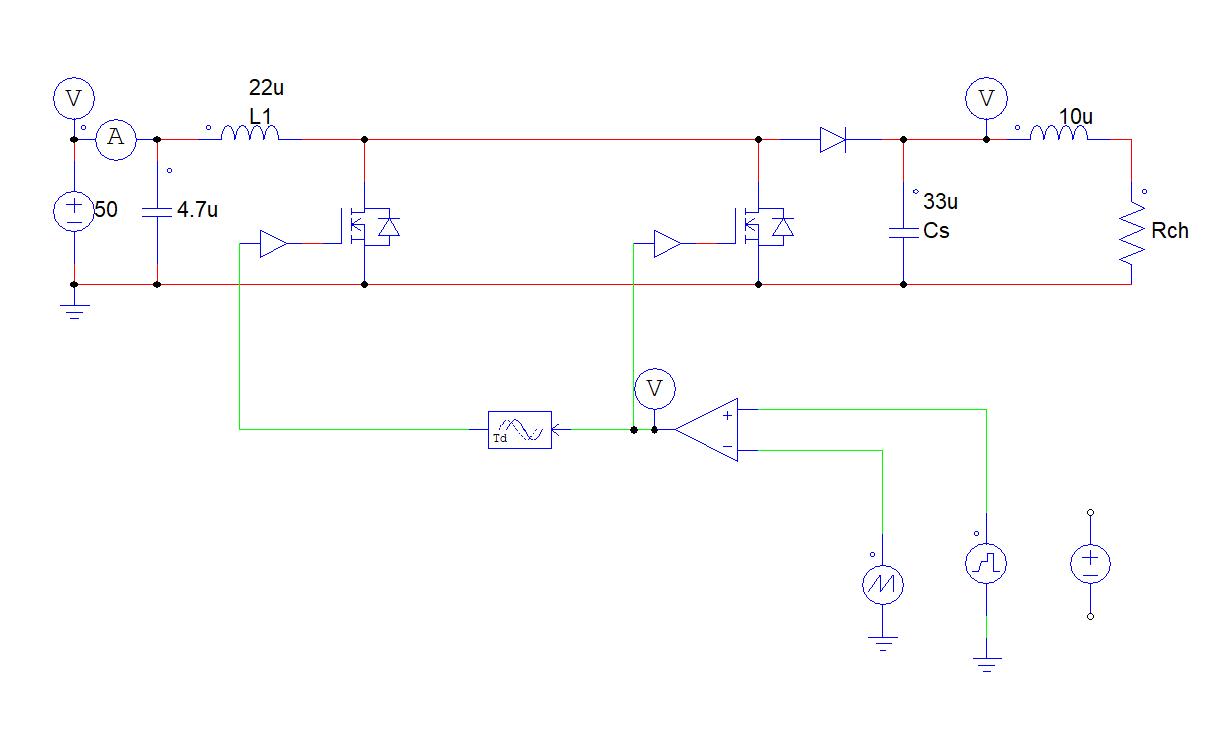
\includegraphics[width=0.8\linewidth]{images/Partie Rice cooker/02_Schéma hacheur dual boost T.png}
    \caption{Schéma Hacheur dual boost en T.}
\end{figure}

Nous devons faire une étude théorique du montage car c'est un montage que nous n'avons pas encore étudié. On commence par réaliser les schémas équivalents pour déterminer les équations pour les deux périodes de fonctionnement~:

\textbf{Entre $0$ et $\alpha T$~:}

\begin{figure}[H]
    \centering
    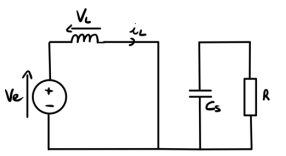
\includegraphics[width=0.8\linewidth]{images/Partie Rice cooker/03_dual boost T petit signaux1.png}
    \caption{Schéma d'étude entre 0 et $\alpha T$, hacheur dual boost en T.}
\end{figure}

\begin{align*}
    V_L(t) &=  V_e \\
    I_L(t) &= \frac{V_e}{L}t + I_{L\text{min}} \\
    V_{T1}(t) &= 0 \\
    i_{T1}(t) &= I_L(t) \\
    V_D(t) &= -V_S \\
    i_{D1}(t) &= 0
\end{align*}

\textbf{Entre $\alpha T$ et $T/2$~:} on pose $t' = t - \alpha T$

\begin{figure}[H]
    \centering
    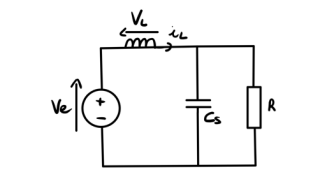
\includegraphics[width=0.8\linewidth]{images/Partie Rice cooker/04_dual boost T petit signaux 2.png}
    \caption{Schéma d'étude entre $\alpha T$ et $T/2$, hacheur dual boost en T.}
\end{figure}

\begin{align*}
    V_L(t') &= V_e - V_s \\
    I_L(t') &= \frac{V_e - V_s}{L}t' + I_{L\text{max}} \\
    V_{T1}(t') &= V_s \\
    i_{T1}(t') &= 0 \\
    V_D(t') &= 0 \\
    i_{D1}(t') &= I_L(t)
\end{align*}

On peut alors écrire (valeur moyenne de la tension aux bornes de l'inductance nulle sur une demi-période)~:

$$ \langle V_L(t) \rangle = 2\alpha V_e + 2\left(\frac{1}{2}-\alpha\right)(V_e - V_s) = 0 $$
$$ 2\alpha V_e + (1-2\alpha)V_e = (1-2\alpha)V_s $$
$$ V_e = (1-2\alpha)V_s $$
$$ \frac{V_s}{V_e} = \frac{1}{1-2\alpha} $$

Avec $V_s = 188~\text{V}$ et $V_e = 50~\text{V}$, on obtient un rapport cyclique $\alpha = 0,367$. \\
En choisissant une ondulation de courant de 100\,\% on obtient la valeur de notre inductance~:

$$ L = \frac{V_e}{I_L \cdot f} = 39~\mu\text{H} $$
$$ I_L = \frac{V_e}{(1-2\alpha)^2 R} = \frac{50}{(1 - 2\cdot0,37)^2 \cdot 78} = 9,48~\text{A} $$
$$ I_{L\text{max}} = I_L + \frac{\Delta I_L}{2} = 11,85~\text{A} $$
$$ I_{L\text{min}} = I_L - \frac{\Delta I_L}{2} = 7,11~\text{A} $$
$$ C_s = \frac{I_L \cdot \alpha}{V_s \cdot f} = \frac{9,48 \cdot 0,37}{28,2 \cdot 100 \cdot 10^3} \approx 1,24~\mu\text{F} \quad \text{(valeur adaptée selon le texte original)}$$

Cette solution a l'avantage de nécessiter assez peu de composants comparée aux autres solutions. Le fonctionnement est le même qu'un hacheur boost sauf que chaque transistor va être piloté par une PWM décalée temporellement d'une demi-période, ce qui aura pour effet de réduire les contraintes thermiques des transistors notamment car ils conduiront le courant sur un temps plus faible chacun (rapport cyclique de $0,37$). La diode et l'inductance vont quant à elles fonctionner à deux fois la fréquence de fonctionnement. Plus on découpe l'énergie souvent (fréquence élevée), moins on a besoin de stocker une grosse quantité d'énergie à chaque cycle. En doublant la fréquence, on peut théoriquement diviser par deux la valeur de l'inductance pour une même ondulation de courant. Donc cela sera un avantage si l'on veut faire un hacheur plus compact.

\textbf{Conclusion générale~:} Nous avons choisi de retenir ces deux topologies de hacheurs pour nos simulations : le hacheur dual boost en T et le hacheur dual boost entrelacé. Nous allons maintenant pouvoir simuler ces deux montages sur PSIM pour voir lequel est le plus économique pour notre application.

\subsubsection*{Simulation PSIM}

\textbf{Hacheur dual boost entrelacé~:}

\begin{figure}[H]
    \centering
    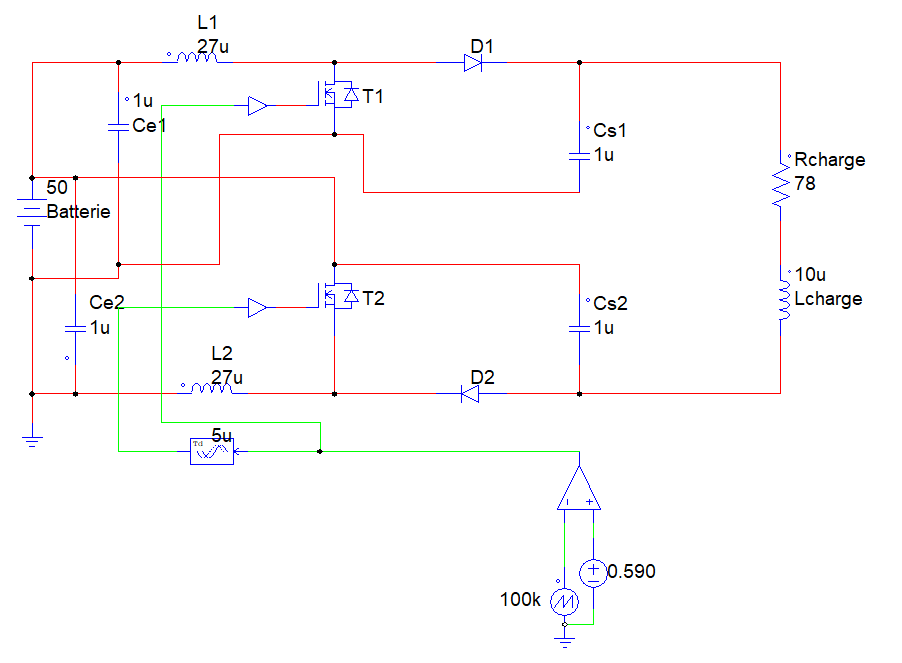
\includegraphics[width=0.8\linewidth]{images/Partie Rice cooker/05_Schéma hacheur entrelacé PSIM.png}
    \caption{Schéma hacheur dual boost entrelacé PSIM.}
\end{figure}

En simulant ce montage avec un rapport cyclique de 0,59, on obtient ceci en sortie de notre convertisseur~:

\begin{figure}[H]
    \centering
    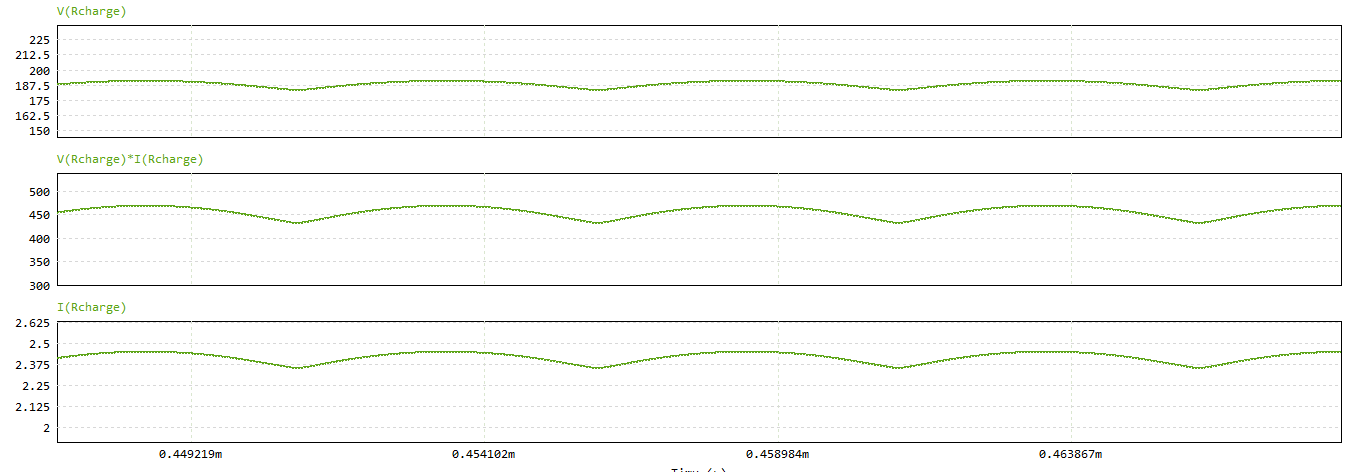
\includegraphics[width=0.8\linewidth]{images/Partie Rice cooker/06_Simulation puissance sortie Hacheur entrelacé.png}
    \caption{Relevé de puissance en sortie du hacheur.}
\end{figure}

Les valeurs de tensions et courants en sortie sont bien conformes à ce que l'on devait obtenir ($187,5~\text{V}$ / $2,4~\text{A}$ / $450~\text{W}$). Cependant, on observe un fort pic au démarrage que l'on pourrait corriger avec une montée progressive du rapport cyclique.

\textbf{Dimensionnement des inductances~:}

Pour dimensionner nos inductances, nous sommes partis de notre valeur calculée qui était de $41~\mu\text{H}$. Ensuite nous avons cherché à diminuer cette valeur afin de réduire la taille du circuit magnétique. La seule condition à respecter était de rester en conduction continue, c'est-à-dire qu'il fallait que la bobine ne décharge pas toute son énergie entièrement à la fin de chaque période. Nous sommes arrivés à une valeur normalisée de $27~\mu\text{H}$ pour laquelle nous étions en limite de conduction comme on peut le voir avec la courbe rouge qui représente l'évolution du courant dans l'inductance en fonction du temps. Ce courant ne passe jamais par 0. On remarque bien que l'inductance se charge et se décharge en fonction de la tension à ses bornes.

\begin{figure}[H]
    \centering
    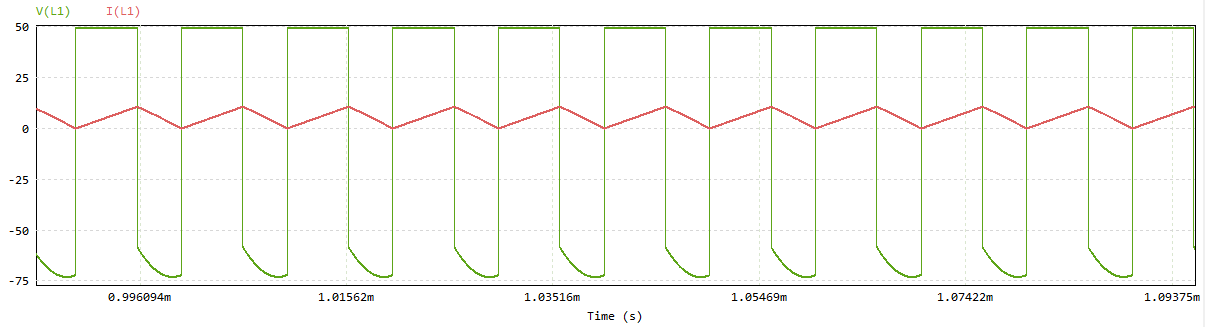
\includegraphics[width=0.8\linewidth]{images/Partie Rice cooker/07_Simulation courant et tension dans la bobine , hacheur entrelacé.png}
    \caption{Relevé courant et tension dans la bobine L1.}
\end{figure}

Pour les condensateurs d'entrée et de sortie, nous sommes restés sur les valeurs calculées car les valeurs obtenues sont acceptables pour la taille des condensateurs.

\textbf{Contraintes sur les composants~:}

\textbf{Condensateurs~:} \\
Le paramètre le plus important à regarder pour les contraintes sur nos condensateurs est le courant qui les traverse. Plus le courant sera grand, plus on devra choisir de gros condensateurs qui prendront plus de place sur notre PCB.

\begin{figure}[H]
    \centering
    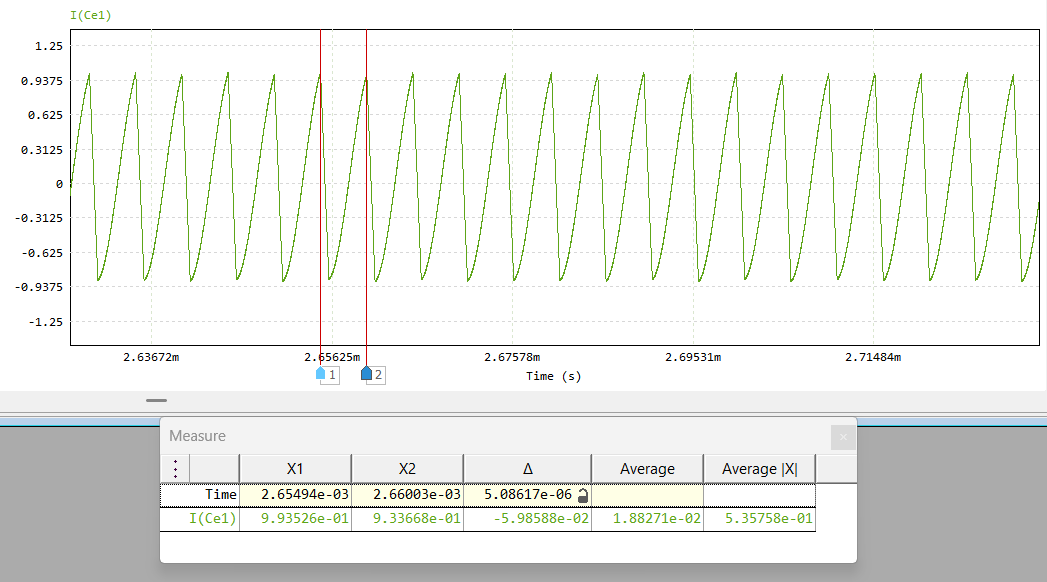
\includegraphics[width=0.8\linewidth]{images/Partie Rice cooker/08_Ice hacheur entrelacé.png}
    \caption{Relevé courant dans la capacité d'entrée du montage Ce1.}
\end{figure}

On relève~:
\begin{itemize}
    \item $I(C_e)$ : $0~\text{A}$ (moyen)
    \item $I(C_e)_{\max}$ : $0,93~\text{A}$
\end{itemize}

\begin{figure}[H]
    \centering
    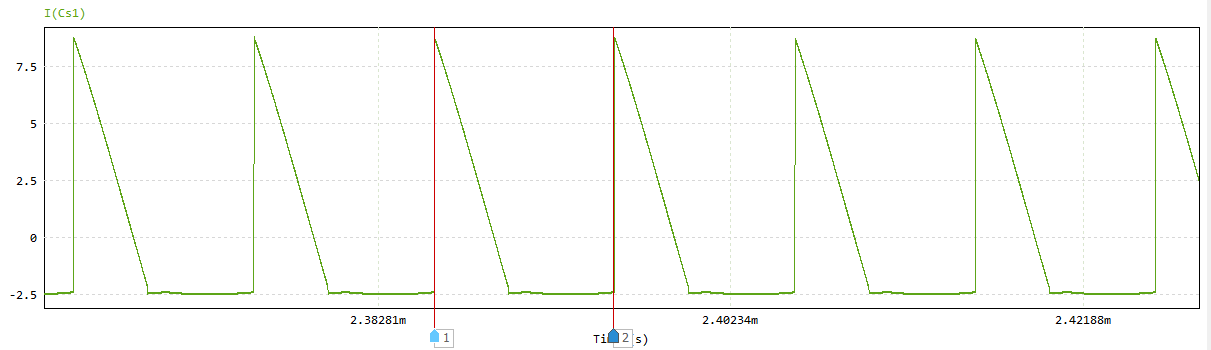
\includegraphics[width=0.8\linewidth]{images/Partie Rice cooker/09_Ics hacheur entrelacé.png}
    \caption{Relevé courant dans la capacité de sortie Cs1.}
\end{figure}

On relève~:
\begin{itemize}
    \item $I(C_s)$ : $2,4~\text{A}$
    \item $I(C_s)_{\max}$ : $8~\text{A}$
\end{itemize}

\textbf{Transistors et diodes~:}

\begin{figure}[H]
    \centering
    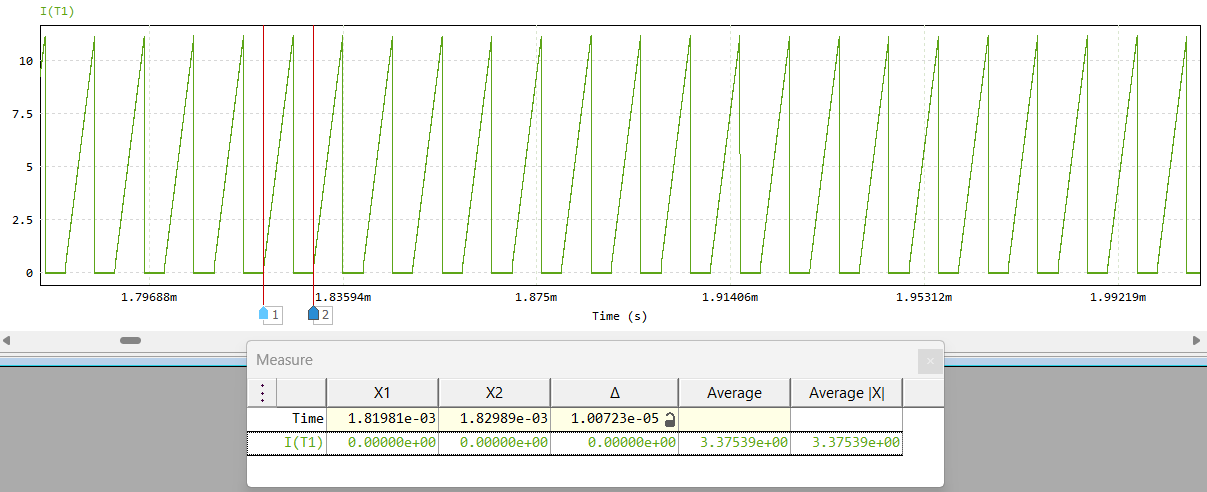
\includegraphics[width=0.8\linewidth]{images/Partie Rice cooker/10_It1 hacheur entrelacé.png}
    \caption{Relevé courant dans le transistor T1.}
\end{figure}

On relève~:
\begin{itemize}
    \item $I(T1)$ : $3,37~\text{A}$
    \item $I(T1)_{\max}$ : $11~\text{A}$
\end{itemize}

\begin{figure}[H]
    \centering
    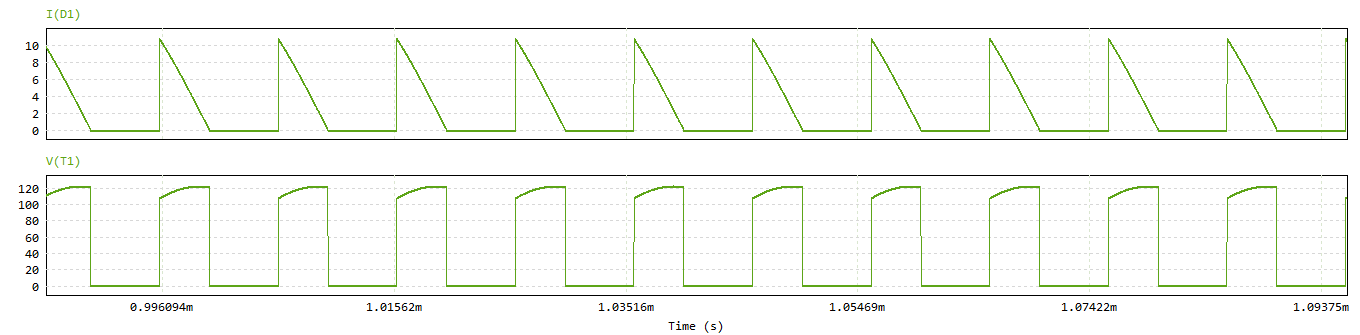
\includegraphics[width=0.8\linewidth]{images/Partie Rice cooker/11_ID1 VT1 hacheur entrelacé.png}
    \caption{Relevé courant dans la diode D1 et tension aux bornes de T1.}
\end{figure}

On relève~:
\begin{itemize}
    \item $I(D1)$ : $2~\text{A}$
    \item $I(D1)_{\max}$ : $11~\text{A}$
    \item $V(T1)$ : $50~\text{V}$
    \item $V(T1)_{\max}$ : $120~\text{V}$
\end{itemize}

\textbf{Hacheur dual boost en T~:}

\begin{figure}[H]
    \centering
    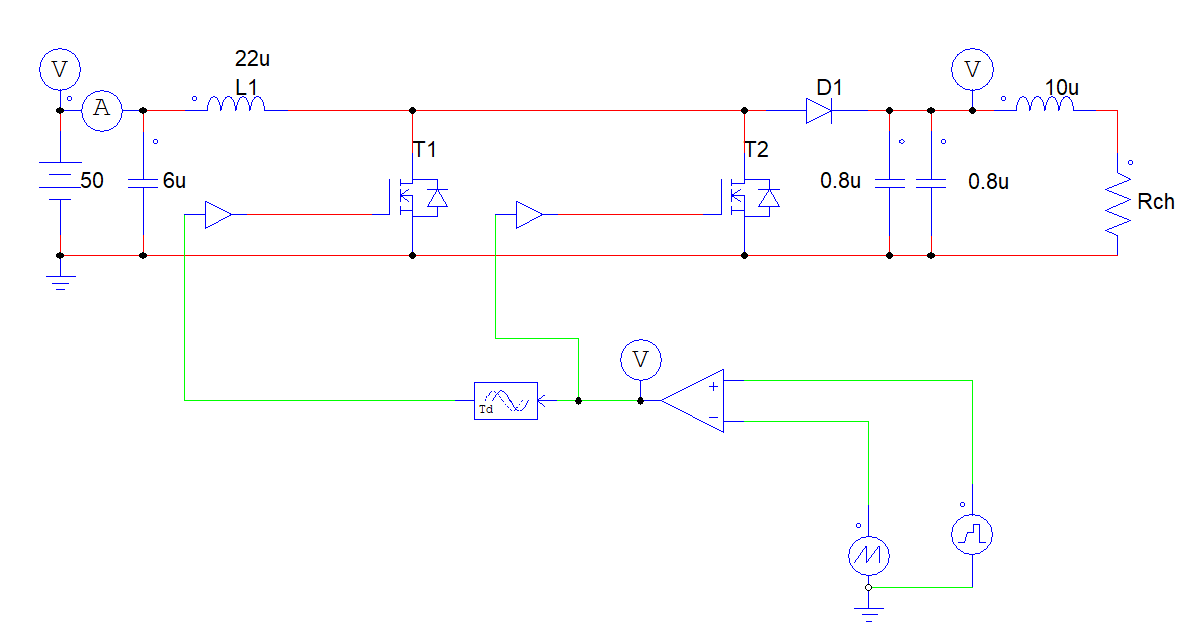
\includegraphics[width=0.8\linewidth]{images/Partie Rice cooker/12_Schéma hacheur dual boost simulation.png}
    \caption{Schéma PSIM avec composants réels, Hacheur dual boost en T.}
\end{figure}

On retrouve ici le schéma étudié précédemment mais avec les composants réels (choisis dans la partie dimensionnement).

En simulant ce montage avec un rapport cyclique de 0,37, on obtient ceci en sortie de notre convertisseur~:

\begin{figure}[H]
    \centering
    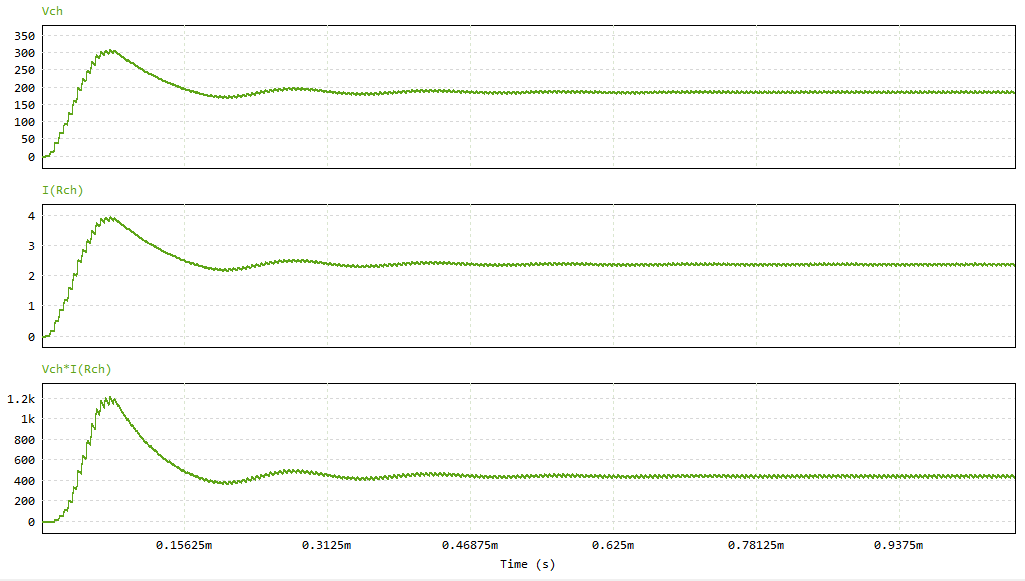
\includegraphics[width=0.8\linewidth]{images/Partie Rice cooker/13_Puissance charge sans rampe.png}
    \caption{Relevé tension, courant et puissance en sortie.}
\end{figure}

Les valeurs de tensions et courants en sortie sont bien conformes à ce que l'on devait obtenir ($187,5~\text{V}$ / $2,4~\text{A}$ / $450~\text{W}$). Cependant, on observe un fort pic au démarrage que l'on pourrait corriger avec une montée progressive du rapport cyclique. On a donc mis en place une montée progressive du rapport cyclique pour ce montage puisque c'est celui que l'on a choisi de mettre en œuvre au final, voici ce que l'on obtient~:

\begin{figure}[H]
    \centering
    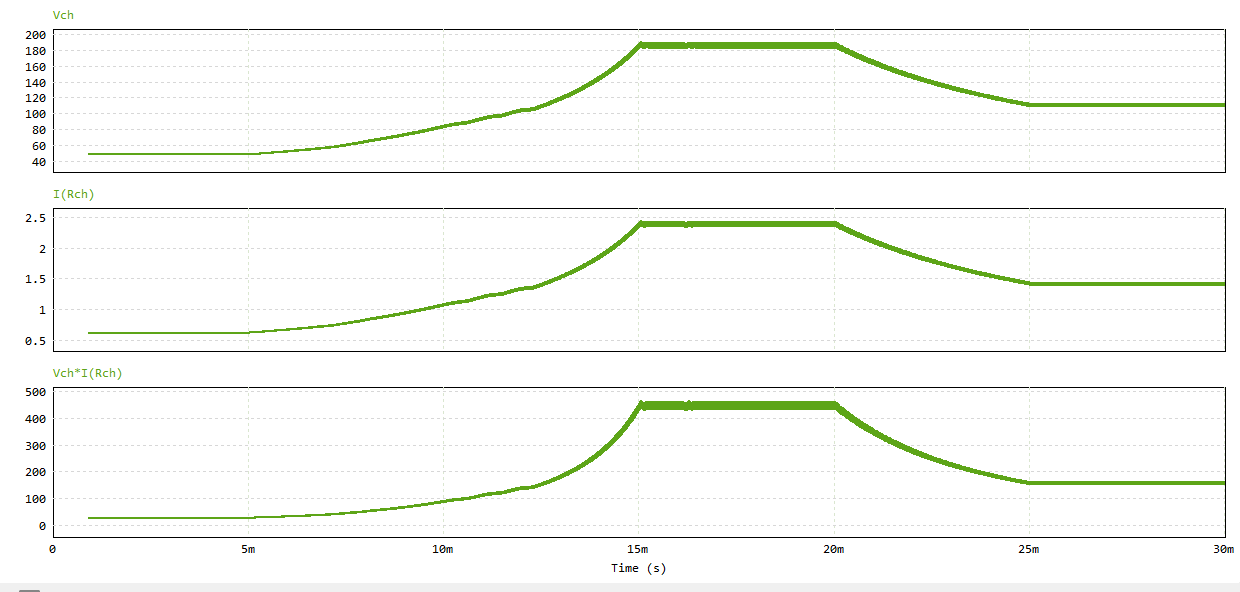
\includegraphics[width=0.8\linewidth]{images/Partie Rice cooker/14_Puissance charge avec rampe.png}
    \caption{Relevé tension, courant et puissance en sortie avec rapport cyclique progressif (rampe).}
\end{figure}

Le pic de puissance lors de la mise sous tension de notre convertisseur a disparu, ce qui nous permet de limiter les contraintes sur nos composants. Nous devrons mettre en place cette mise sous tension douce à l'aide d'un code dans notre PIC qui va contrôler les signaux PWM des transistors.

\textbf{Dimensionnement de l'inductance L~:} \\
Pour dimensionner nos inductances, nous sommes partis de la valeur calculée comme pour le montage précédent et on a diminué la valeur au minimum tout en restant en conduction continue. Nous obtenons une valeur de $22~\mu\text{H}$ en valeur normalisée.

\textbf{Contraintes sur les composants~:}

\textbf{Condensateurs~:}

\begin{figure}[H]
    \centering
    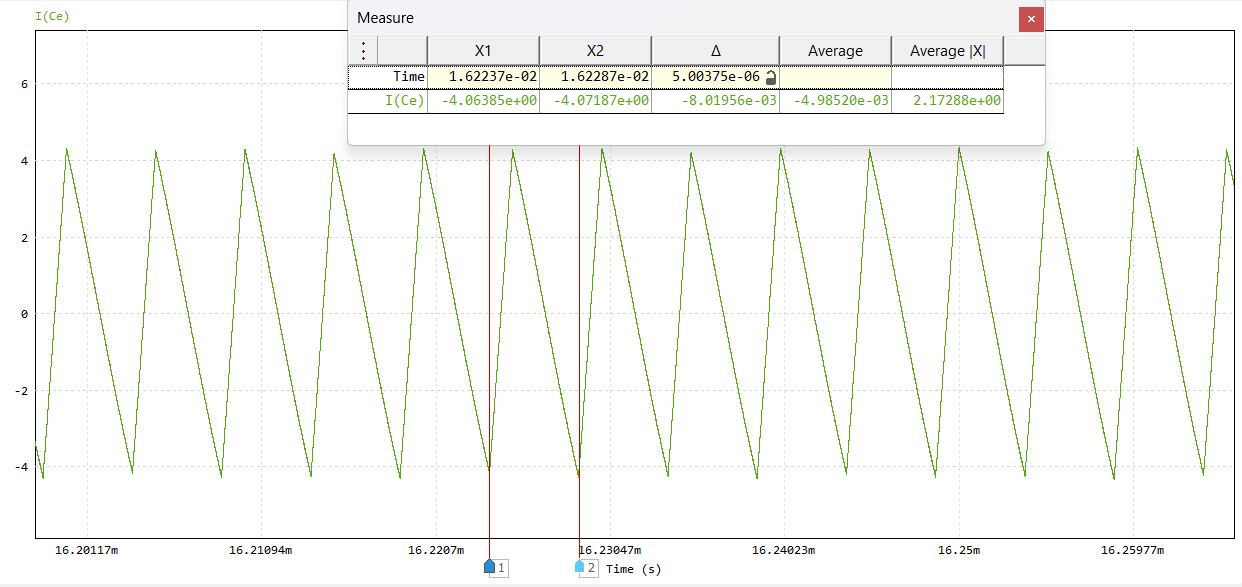
\includegraphics[width=0.8\linewidth]{images/Partie Rice cooker/15_Ice d.png}
    \caption{Relevé courant dans la capacité d'entrée Ce.}
\end{figure}

On relève~:
\begin{itemize}
    \item $I(C_e)$ : $2,17~\text{A}$
    \item $I(C_e)_{\max}$ : $4,2~\text{A}$
\end{itemize}

\begin{figure}[H]
    \centering
    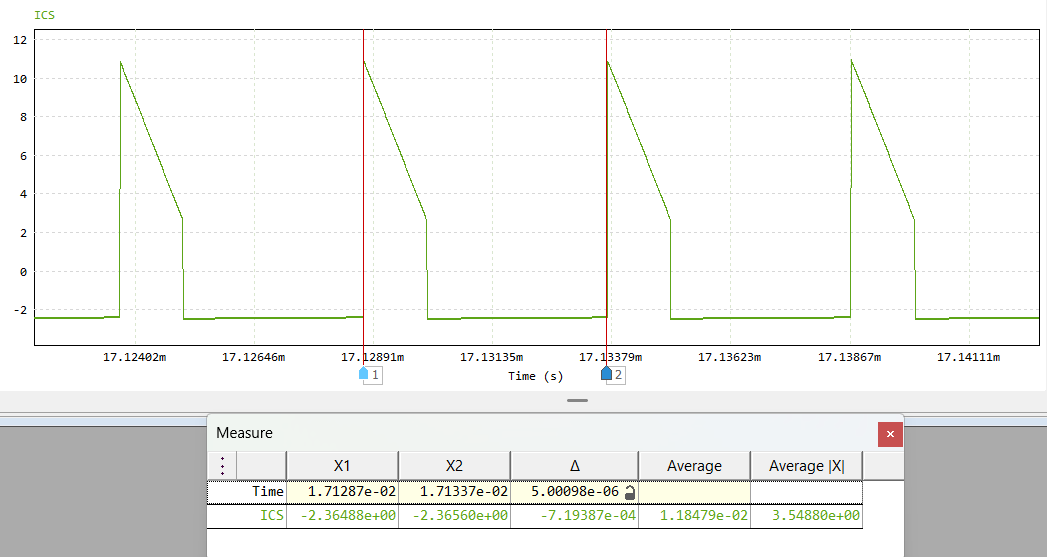
\includegraphics[width=0.8\linewidth]{images/Partie Rice cooker/16_Ics.png}
    \caption{Relevé courant dans la capacité de sortie Cs.}
\end{figure}

On relève~:
\begin{itemize}
    \item $I(C_s)$ : $3,55~\text{A}$
    \item $I(C_s)_{\max}$ : $11~\text{A}$
\end{itemize}

\textbf{Transistor et diodes~:}

\begin{figure}[H]
    \centering
    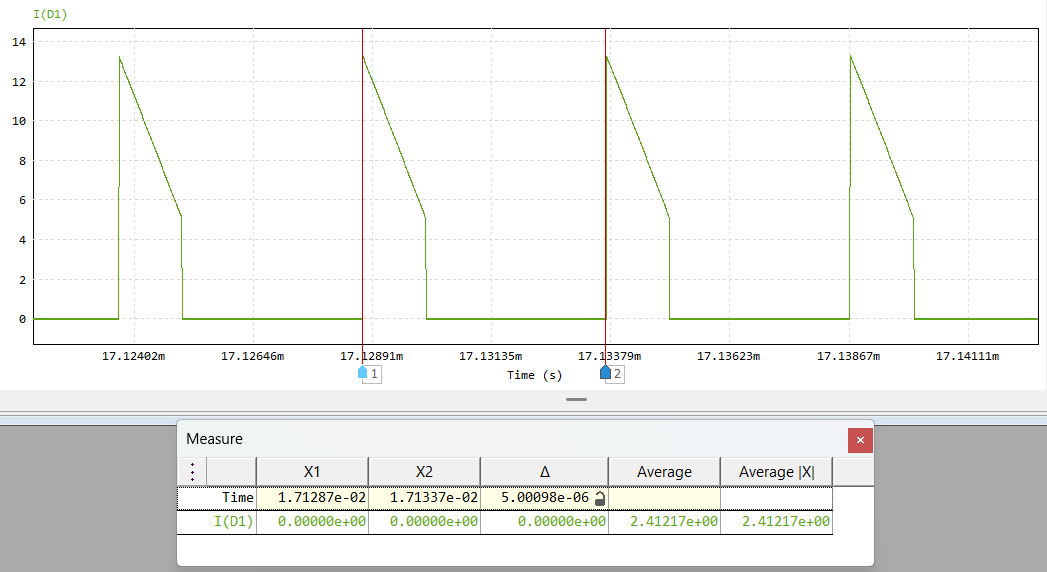
\includegraphics[width=0.8\linewidth]{images/Partie Rice cooker/17_ID1.png}
    \caption{Relevé courant dans la diode D1.}
\end{figure}

On relève~:
\begin{itemize}
    \item $I(D1)$ : $2,4~\text{A}$
    \item $I(D1)_{\max}$ : $13~\text{A}$
\end{itemize}

\begin{figure}[H]
    \centering
    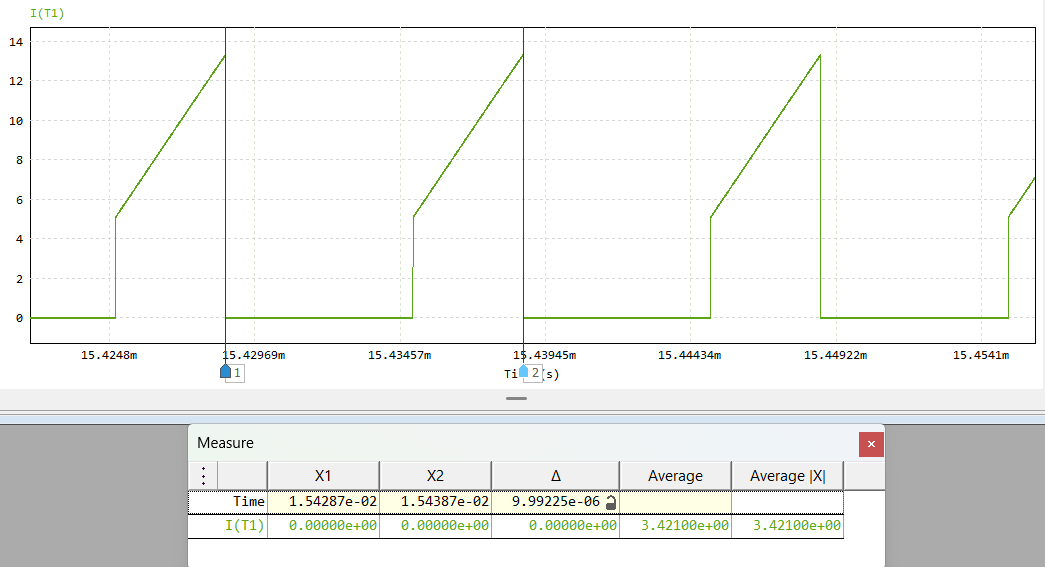
\includegraphics[width=0.8\linewidth]{images/Partie Rice cooker/18_IT1.png}
    \caption{Relevé courant dans le transistor T1.}
\end{figure}

On relève~:
\begin{itemize}
    \item $I(T1)$ : $3,42~\text{A}$
    \item $I(T1)_{\max}$ : $13~\text{A}$
\end{itemize}

\begin{figure}[H]
    \centering
    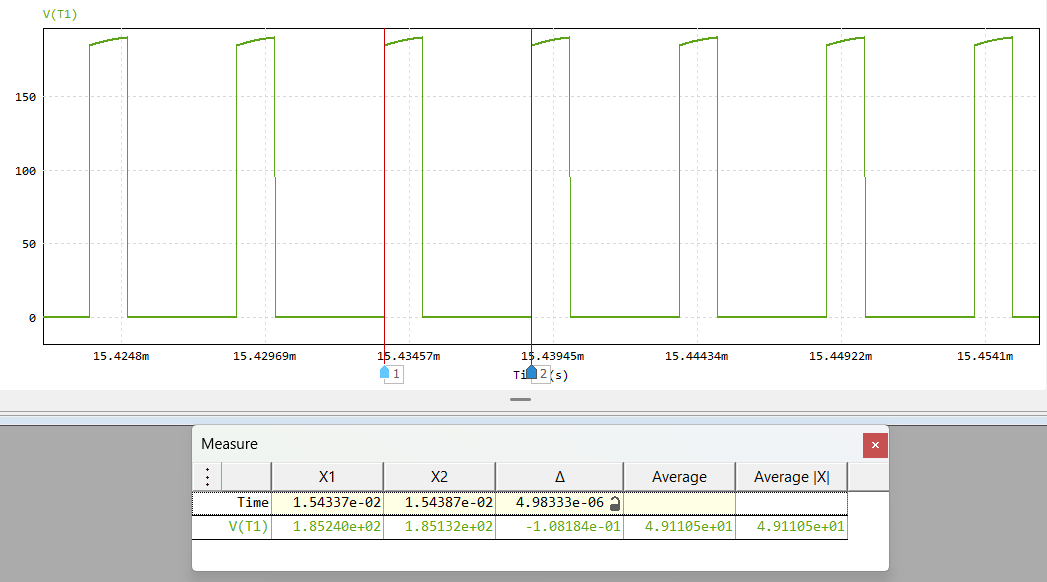
\includegraphics[width=0.8\linewidth]{images/Partie Rice cooker/19_VT1.png}
    \caption{Tension aux bornes du transistor T1.}
\end{figure}

On relève~:
\begin{itemize}
    \item $V(T1)$ : $49~\text{V}$
    \item $V(T1)_{\max}$ : $195~\text{V}$
\end{itemize}

\textbf{Tableau récapitulatif des contraintes sur les composants~:}

\begin{tableau}[H]
    \centering
    \begin{tabular}{|p{3cm}|p{6cm}|p{6cm}|}
    \hline
    \textbf{Composants} & \textbf{Hacheur dual boost entrelacé} & \textbf{Hacheur dual boost en T} \\
    \hline
    \textbf{Transistors MOSFET} & Courant moyen : $3,37~\text{A}$ \newline Pic de courant : $11~\text{A}$ \newline Tension moyenne : $50~\text{V}$ \newline Pic de tension : $120~\text{V}$ & Courant moyen : $3,42~\text{A}$ \newline Pic de courant : $13~\text{A}$ \newline Tension moyenne : $49~\text{V}$ \newline Pic de tension : $195~\text{V}$ \\
    \hline
    \textbf{Diodes} & Courant moyen : $2~\text{A}$ \newline Pic de courant : $11~\text{A}$ & Courant moyen : $2,4~\text{A}$ \newline Pic de courant : $13~\text{A}$ \\
    \hline
    \textbf{Condensateurs entrée} & Courant moyen : $0~\text{A}$ \newline Pic de courant : $0,93~\text{A}$ & Courant moyen : $2,17~\text{A}$ \newline Pic de courant : $4,2~\text{A}$ \\
    \hline
    \textbf{Condensateurs sortie} & Courant moyen : $2,4~\text{A}$ \newline Pic de courant : $8~\text{A}$ & Courant moyen : $3,55~\text{A}$ \newline Pic de courant : $11~\text{A}$ \\
    \hline
    \end{tabular}
    \caption{Récapitulatif des contraintes.}
\end{tableau}

\textbf{Analyse~:} Le principal avantage que l'on aura avec la structure entrelacée est que la contrainte de tension sur les MOSFETs est de $120~\text{V}$ contre $195~\text{V}$ pour la structure en T. Plus la tension nominale d'un MOSFET est élevée, plus sa résistance à l'état passant $R_{\text{Dson}}$ est grande, ce qui génère plus de pertes par conduction et fait chauffer le composant. On aura le choix entre deux gammes : $150~\text{V}$ ou $250~\text{V}$. Cependant dans notre cas, si on choisit la structure entrelacée, la gamme $150~\text{V}$ est un peu juste car on a peu de marge par rapport à la surtension au blocage due à l'inductance du circuit ($30~\text{V}$), donc on devra choisir la gamme au-dessus ($250~\text{V}$). Au final, pour le choix des transistors, les deux structures ne présentent pas de net avantage. En ce qui concerne les autres composants (diodes et condensateurs), la structure entrelacée permet d'obtenir des courants crêtes moins élevés pour les condensateurs et les diodes, mais il n'y a pas d'énormes différences entre les valeurs qui nous pousseraient à choisir cette structure plutôt que le hacheur en T.

\textbf{Choix de la solution technique~:}

Au regard des calculs théoriques et des simulations effectuées, pour obtenir le meilleur compromis sur le plan économique, le nombre de composants, la facilité de mise en œuvre tout en ayant une structure qui fonctionne pour notre application (faire chauffer une résistance, tout simplement), nous avons choisi le \textbf{hacheur dual boost en T} car il présente des avantages en termes de facilité de réalisation~: pas d'entrelacement qui rendrait le PCB plus complexe avec des pistes qui se croisent, moins de composants donc une solution moins chère et pour notre application, ce montage suffit amplement.

        \subsection{Choix des composants}

\subsubsection*{Partie puissance}

\textbf{Transistor~:} Ref~: IMT65R039M1HXUMA1 \\
\textbf{Diode~:} Ref~: V35PW22HM3/I

Dans le cadre de la gestion globale du projet et afin d'optimiser les coûts via une stratégie d'achats groupés à l'échelle de la classe, les références des semi-conducteurs de puissance nous ont été imposées.

\textbf{Bobine~:} Ref~: SRP1770TA-220M

\begin{figure}[H]
    \centering
    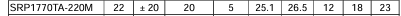
\includegraphics[width=0.8\linewidth]{images/Partie Rice cooker/20_bobine caractéristiques.png}
    \caption{Caractéristiques bobine L1.}
\end{figure}

\begin{figure}[H]
    \centering
    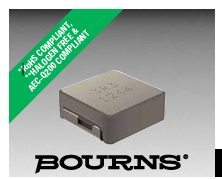
\includegraphics[width=0.5\linewidth]{images/Partie Rice cooker/21_bobine aspect extérieur.png}
    \caption{Aspect extérieur bobine L1.}
\end{figure}

Composant plus qu'important pour le stockage d'énergie, cette bobine a été choisie pour ses performances élevées et sa compacité. Ses caractéristiques répondent précisément à nos besoins~:
\begin{itemize}
    \item \textbf{Tenue en courant~:} Avec un courant efficace admissible de $12~\text{A}$ et un courant de saturation de $18~\text{A}$, elle supporte largement notre courant moyen de $9,48~\text{A}$ et nos pics de courant calculés à $11,85~\text{A}$.
\end{itemize}

\textbf{Condensateur d'entrée~:}

\begin{figure}[H]
    \centering
    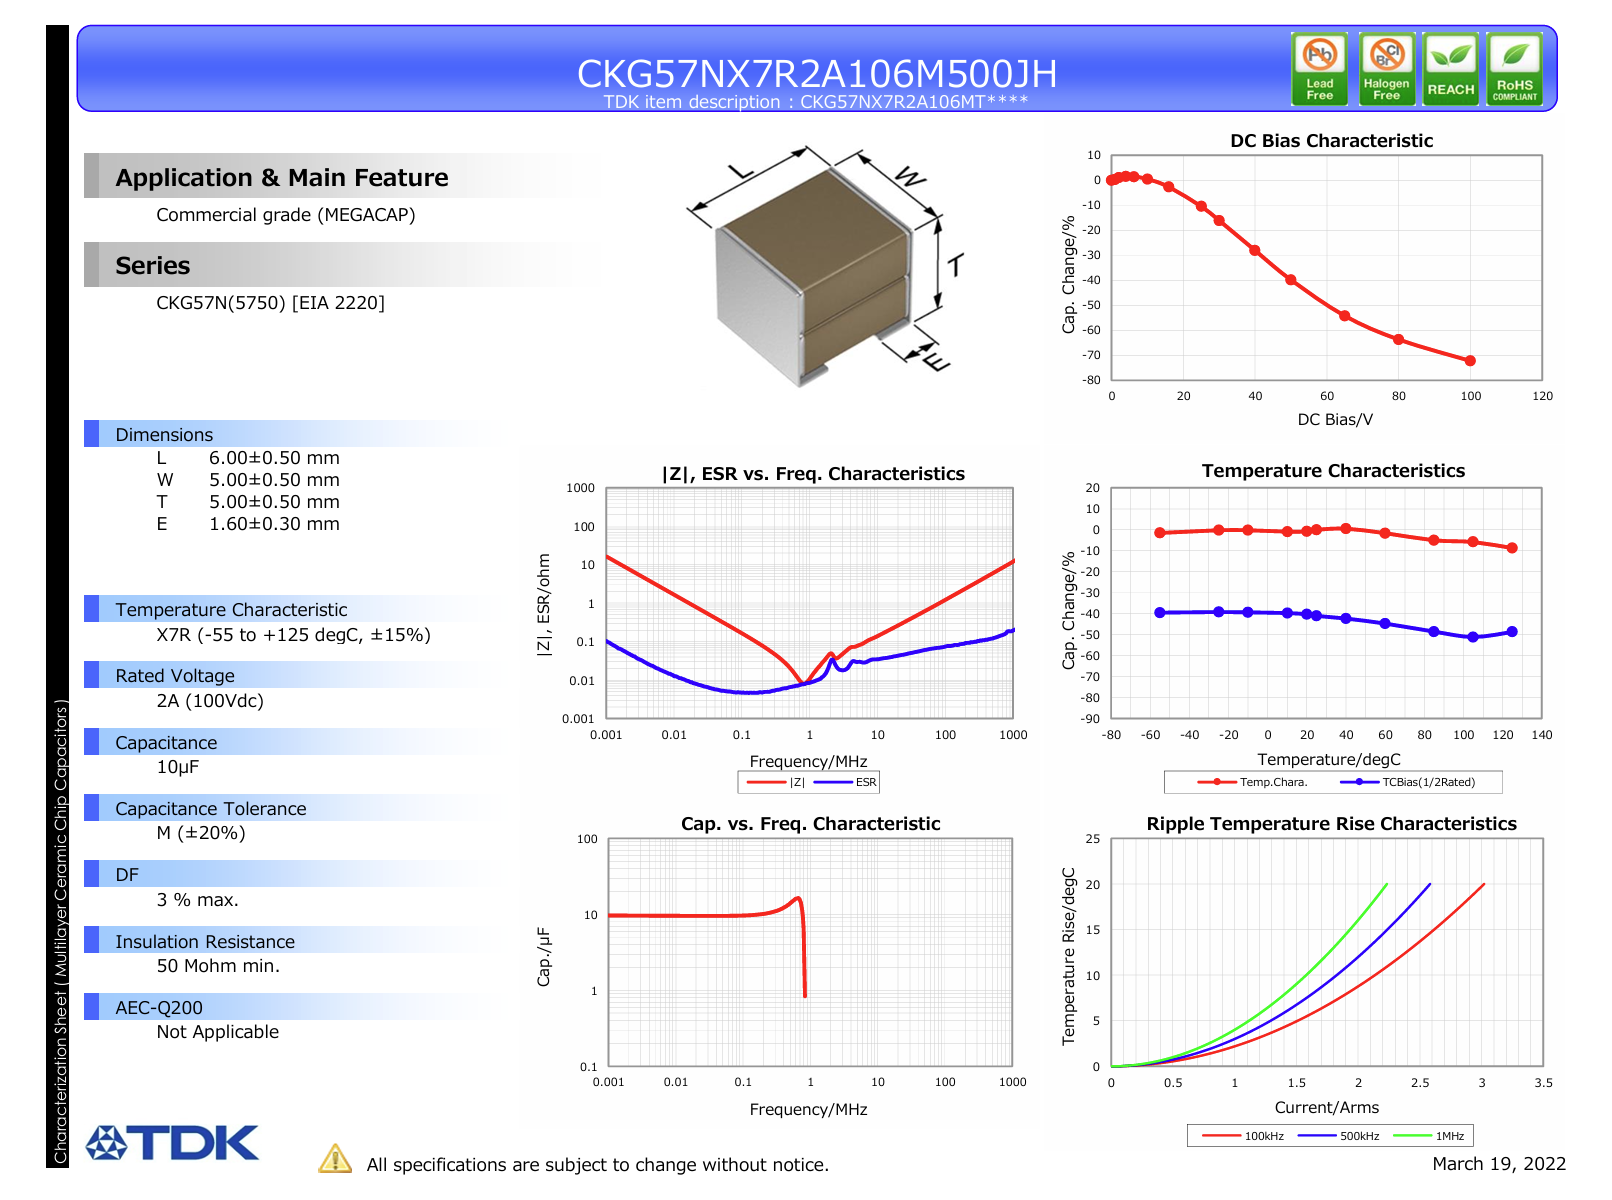
\includegraphics[width=0.8\linewidth]{images/Partie Rice cooker/22_capacité d_entrée.png}
    \caption{Caractéristiques capacité d'entrée.}
\end{figure}

Nous avons choisi un condensateur X7R (céramiques de classe II) pour l'entrée car, à $50~\text{V}$, un X7R perdra de la capacité, mais cela reste gérable. Les céramiques multi-couches de Classe II offrent le meilleur équilibre entre la taille, les performances à haute fréquence et la capacité de gestion du courant, face aux autres technologies disponibles.

Le choix de la référence CKG57NX7R2A106M500JH ($10~\mu\text{F}$ nominal) a été dicté par la nécessité de maintenir un réservoir d'énergie local stable malgré les contraintes de fonctionnement du hacheur.

\textbf{Prise en compte de la chute de la capacité~:} L'analyse de la courbe de caractéristique "DC Bias" montre qu'un condensateur céramique perd une partie de sa capacité lorsqu'il est soumis à une tension continue. Sous notre tension d'entrée de $50~\text{V}$, la capacité effective chute de 40\,\%, nous laissant avec une valeur réelle de $6~\mu\text{F}$ en fonctionnement.

Nous avons alors utilisé cette valeur de $6~\mu\text{F}$ lors des simulations.

\textbf{Condensateur de sortie~:}

\begin{figure}[H]
    \centering
    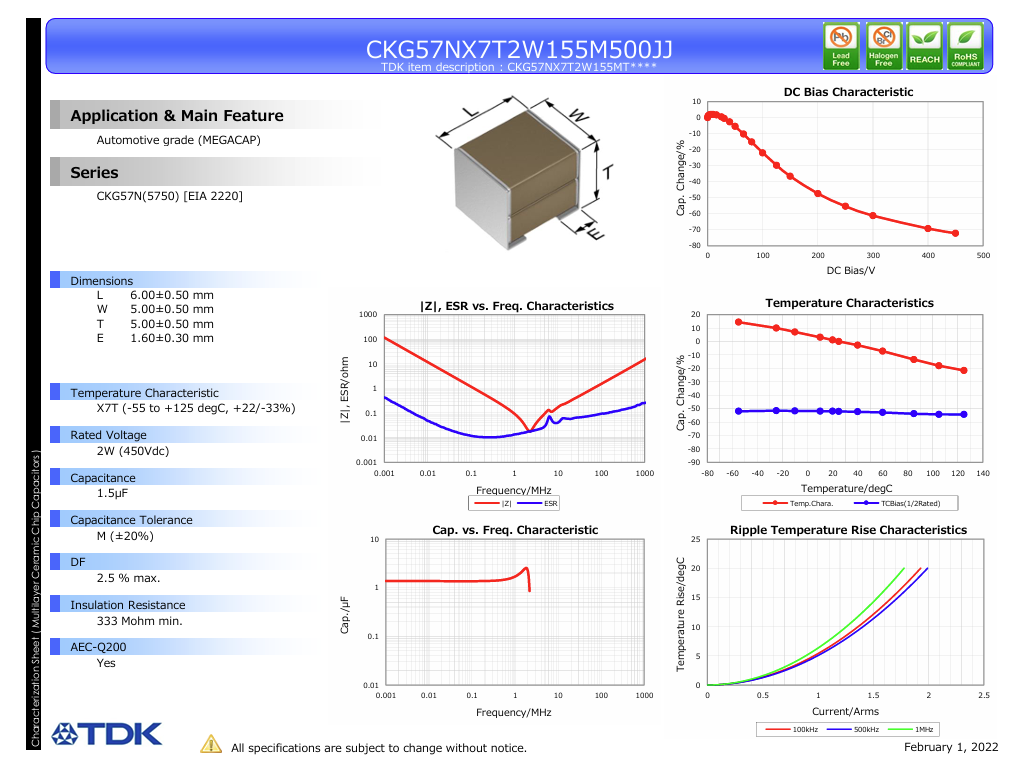
\includegraphics[width=0.8\linewidth]{images/Partie Rice cooker/23_Capacité de sortie.png}
    \caption{Caractéristiques capacité de sortie.}
\end{figure}

Nous avons choisi un condensateur X7T pour la sortie car il permet d'utiliser une valeur nominale de départ très élevée dans un boîtier standard. Ainsi, même après s'être effondrée sous l'effet des $188~\text{V}$ (DC Bias), la capacité restante est toujours suffisante. Le X7R ne permettrait tout simplement pas d'obtenir cette capacité résiduelle sans démultiplier la taille ou le nombre de composants.

Le dimensionnement théorique a établi qu'une capacité minimale de $1,24~\mu\text{F}$ était nécessaire pour limiter l'ondulation de la tension de sortie.

Cependant, l'analyse de la datasheet de notre référence (CKG57NX7T2W155M500JJ) montre qu'à notre tension de service de $188~\text{V}$, la capacité effective chute à environ $0,8~\mu\text{F}$ par composant en raison du phénomène de DC Bias.

Pour compenser cette perte de caractéristique, nous avons choisi de placer deux condensateurs en parallèle, comme illustré sur notre schéma de simulation. Cette configuration nous permet d'atteindre une capacité réelle totale de $1,6~\mu\text{F}$. Cette valeur étant supérieure aux $1,24~\mu\text{F}$ requis par le calcul, elle garantit non seulement le respect du cahier des charges sur l'ondulation de tension, mais offre également une marge de sécurité supplémentaire pour la stabilité de la sortie.

\subsubsection*{Partie commande}

\textbf{Convertisseur 5V / 15V~:} Ref~: SCT01F05S15

\textbf{Filtre 5V / 15V~:} \\
En étudiant la documentation technique du convertisseur, nous avons observé que le constructeur recommandait de créer un filtre composé d'une bobine et d'une capacité en entrée.

\begin{figure}[H]
    \centering
    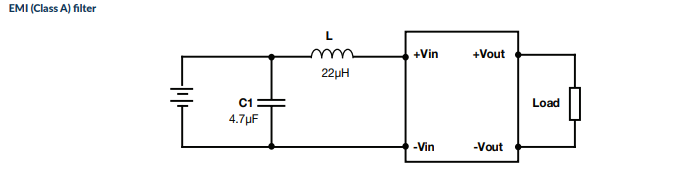
\includegraphics[width=0.8\linewidth]{images/Partie Rice cooker/24_Filtre classe A 5 15.png}
    \caption{Filtre conseillé par le constructeur.}
\end{figure}

\textbf{Bobine filtre~:} Ref~: LQH32PN220MN0L \\
Cette référence présente un excellent compromis~: elle offre l'inductance requise de $22~\mu\text{H}$ tout en garantissant une faible résistance série (DCR). Cela permet de limiter les chutes de tension et les pertes par effet Joule en entrée du convertisseur. De plus, son courant de saturation est largement supérieur à la consommation d'entrée du module, évitant tout risque de perte d'inductance en charge.

\textbf{Capacité filtre~:} Ref~: C1206C475M3RACTU \\
Conformément aux préconisations du constructeur pour le filtre EMI Classe A, nous avons choisi une capacité de $4,7~\mu\text{F}$. Notre choix s'est porté sur un condensateur céramique multicouche de chez KEMET. Afin de garantir une bonne fiabilité et de limiter l'effet de perte de capacité sous tension continue, nous avons opté pour un modèle supportant une tension de $25~\text{V}$ (pour une utilisation sous $5~\text{V}$).

\begin{figure}[H]
    \centering
    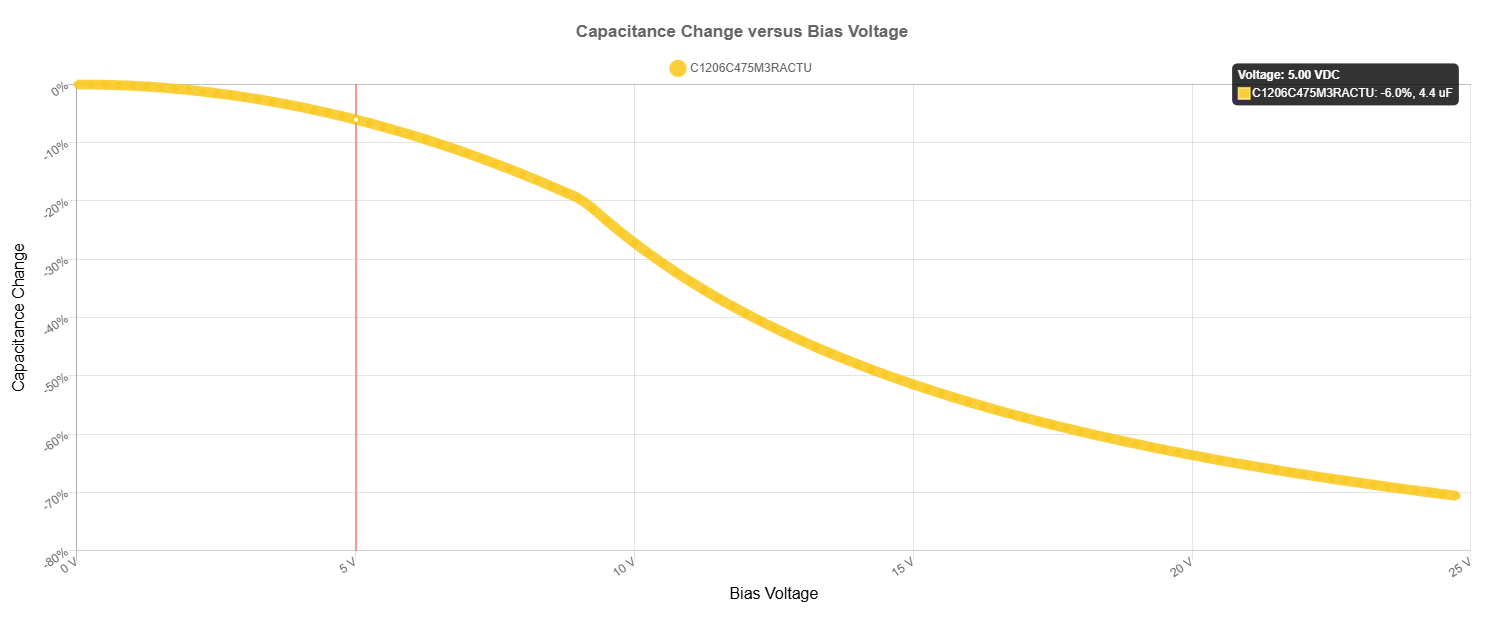
\includegraphics[width=0.8\linewidth]{images/Partie Rice cooker/25_Courbe chute capacité en fonction de la tension ( 5_15 filtre).PNG}
    \caption{Chute de la valeur de la capacité du filtre en fonction de la tension (DC).}
\end{figure}

\textbf{Capacité de découplage~:} Ref~: C3216X7R1H106K160AC \\
Des condensateurs de découplage sont placés au plus près des composants actifs (PIC, drivers) pour filtrer les parasites et stabiliser la tension locale. Notre choix s'est porté sur ce modèle CMS pour plusieurs raisons~:
\begin{itemize}
    \item \textbf{Valeur ($10~\mu\text{F}$)~:} Offre un réservoir d'énergie suffisant pour absorber les appels de courant transitoires liés aux commutations rapides.
    \item \textbf{Format CMS (1206)~:} Réduit considérablement l'inductance parasite (ESL), ce qui est indispensable pour un bon filtrage haute fréquence.
    \item \textbf{Tension de $50~\text{V}$~:} Limite fortement le phénomène de DC Bias (perte de capacité sous tension continue), garantissant que les $10~\mu\text{F}$ restent effectifs sous $5~\text{V}$ ou $15~\text{V}$.
    \item \textbf{Diélectrique X7R~:} Assure une grande stabilité de la capacité face aux variations de température du système.
\end{itemize}

        \subsection{Schéma détaillé et PCB}

Après avoir réalisé les différentes simulations que nous avons détaillées précédemment nous sommes passés à la partie réalisation du/des PCB. \\
Dans un premier temps, nous voulions séparer la partie commande de la partie puissance pour faciliter la création de deux PCBs plus petits mais plus faciles à réaliser et à souder. \\
Cependant, pour avoir les meilleures performances possibles, nous nous sommes dirigés vers la réalisation d'un seul PCB. Celui-ci permettra alors, en ayant notamment les drivers au plus proche possible des transistors, une meilleure efficacité. \\
Malgré cela, ce PCB reste plus compliqué à réaliser au vu du nombre de composants, de connexions ou encore des différences de type de composants (CMS et Traversants).

\textbf{Schéma Proteus~:}

\begin{figure}[H]
    \centering
    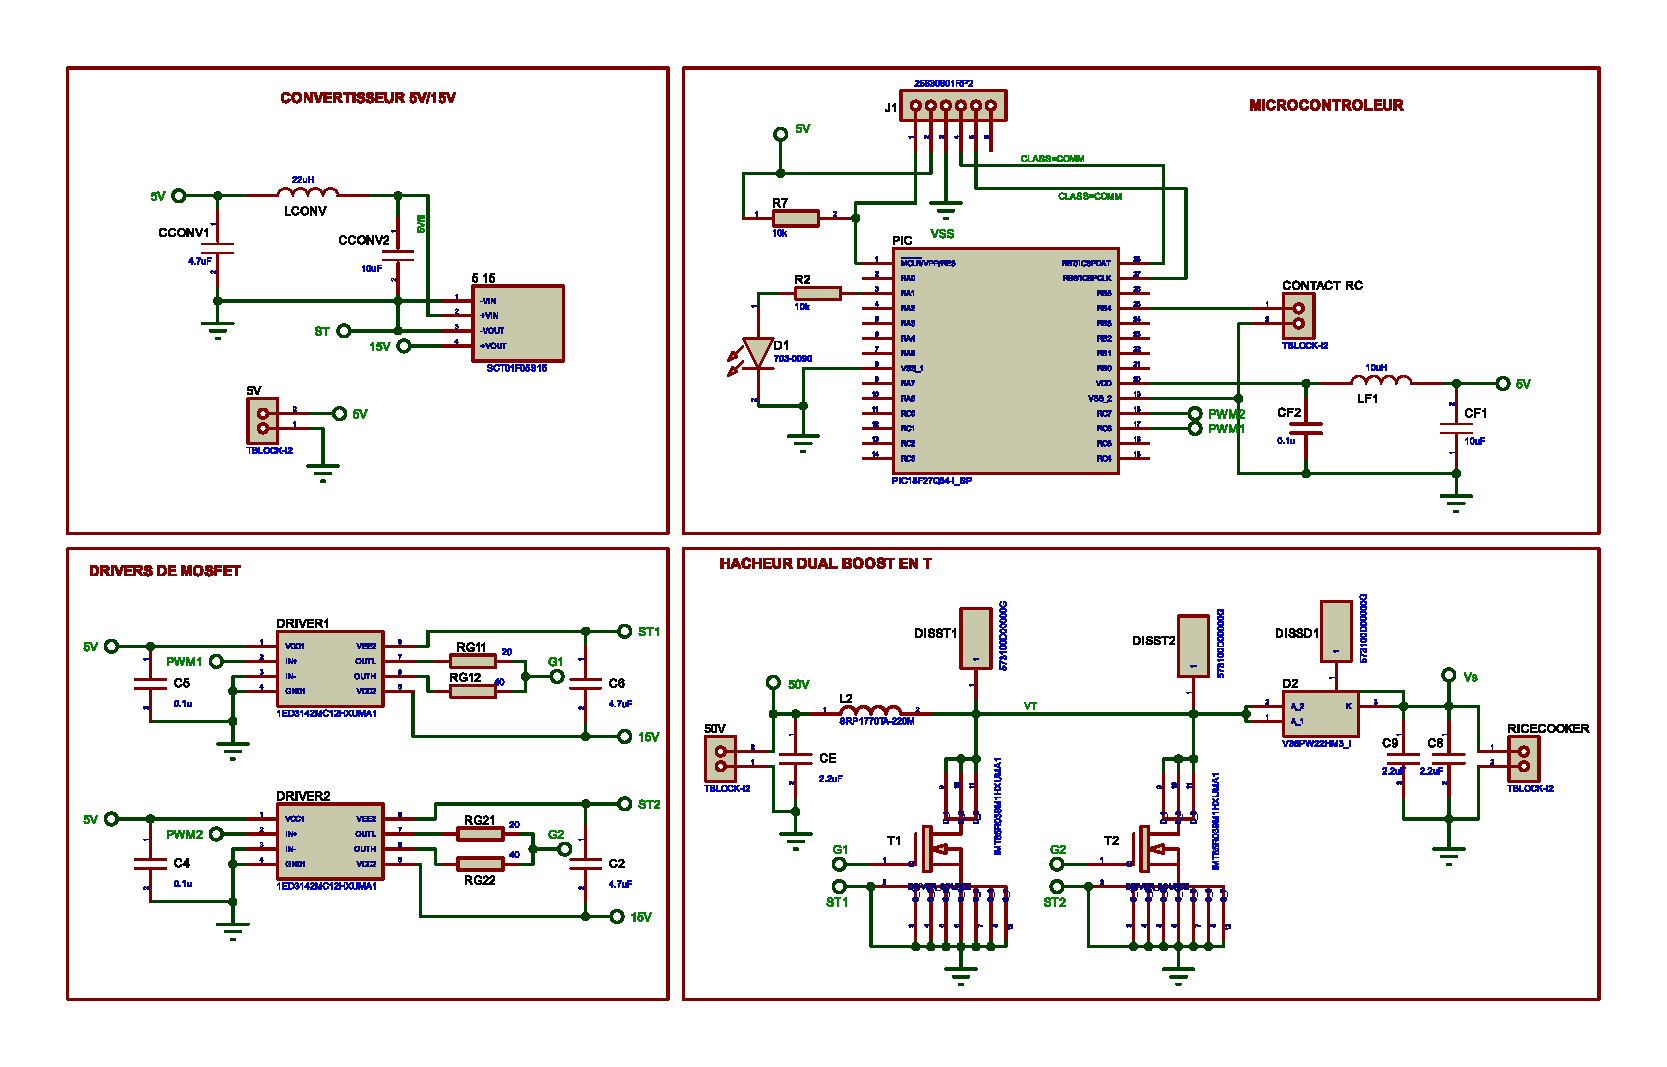
\includegraphics[width=1\linewidth]{images/Partie Rice cooker/26_SCHEMA PROTEUS VERSION1.pdf}
    \caption{Schéma Proteus.}
\end{figure}

\textbf{PCB première version~:}

\begin{figure}[H]
    \centering
    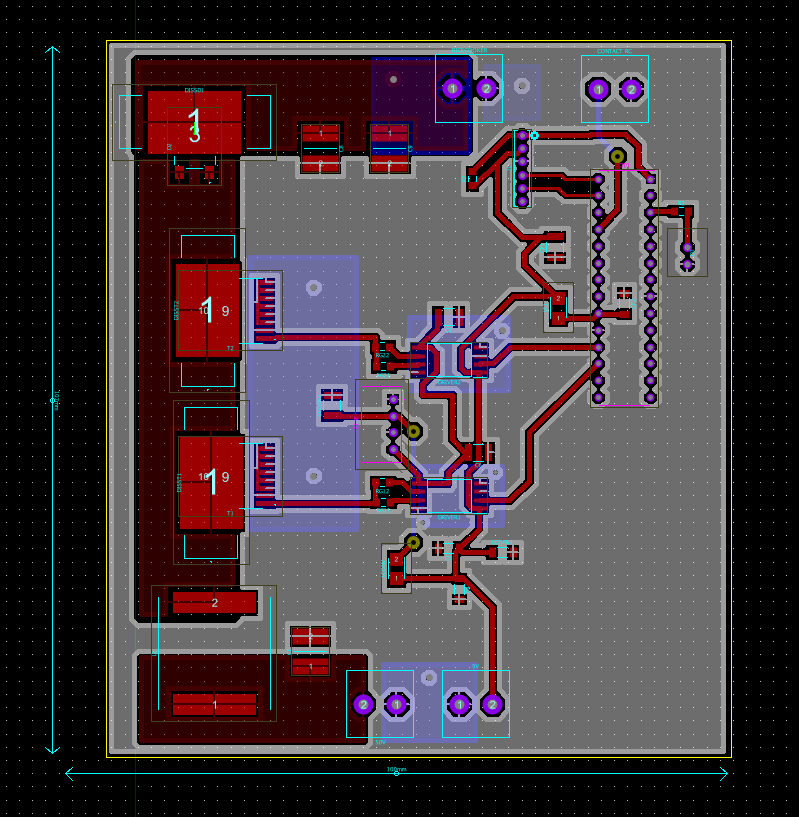
\includegraphics[width=0.8\linewidth]{images/Partie Rice cooker/27_PCB VERSION 1.PNG}
    \caption{PCB version 1.}
\end{figure}

Cette première version permet de se rendre compte des différentes problématiques énoncées précédemment, mais également du fait qu'il faut prévoir de la place pour la dissipation thermique autour des transistors et de la diode. L'objectif est d'améliorer ce PCB jusqu'à arriver à une version finale.

        \subsection{Adaptation Rice-cooker}

Comme décrit dans l'analyse fonctionnelle, notre rice cooker doit répondre à ces deux points~:
\begin{itemize}
    \item \textbf{Modulation~:} L'alimentation doit être "modulable" pour faire varier la puissance de chauffe en fonction du mode désiré (cuisson et maintien en température).
    \item \textbf{Adaptation~:} Fonctionnement en tension continue au lieu d'une tension alternative provenant du réseau (230~Vac).
\end{itemize}

Nous avons choisi d'utiliser un microcontrôleur PIC qui détectera l'impulsion déclenchée par l'ouverture du contact du switch magnétique qui se désaimante lorsque la température ciblée est atteinte. Dans le cas du circuit de base présent dans notre appareil, on bascule dans ce cas sur une plus petite résistance qui dissipe moins de chaleur afin de maintenir les aliments au chaud.

Dans notre nouveau circuit, on va enlever cette résistance car elle ne sera pas nécessaire puisque la puissance dissipée sera contrôlée uniquement par les PWM de notre microcontrôleur, donc on utilisera seulement la grosse résistance.

Nous allons séparer la partie alimentation là où tout le courant va circuler dans la résistance de charge de la partie détection qui va se brancher sur notre PIC afin de ne pas détruire celui-ci (il ne supporterait pas des tensions aussi élevées).

Cela pose un problème puisque la LED qui indique le maintien au chaud des aliments n'est ainsi plus alimentée par les 188~Vdc (cette LED a besoin d'une tension d'alimentation d'au moins 120~Vdc pour s'allumer d'après les tests que l'on a effectués). Nous devrons donc utiliser une petite LED de la même couleur qui pourra s'allumer avec les 5~V de notre microcontrôleur PIC et qui va remplir la même fonction.

Une résistance de pull-up sera placée afin de définir un état logique clair et stable sur la broche d'entrée de notre PIC lorsque l'interrupteur n'est pas actionné et ne pas avoir d'état flottant.

\begin{figure}[H]
    \centering
    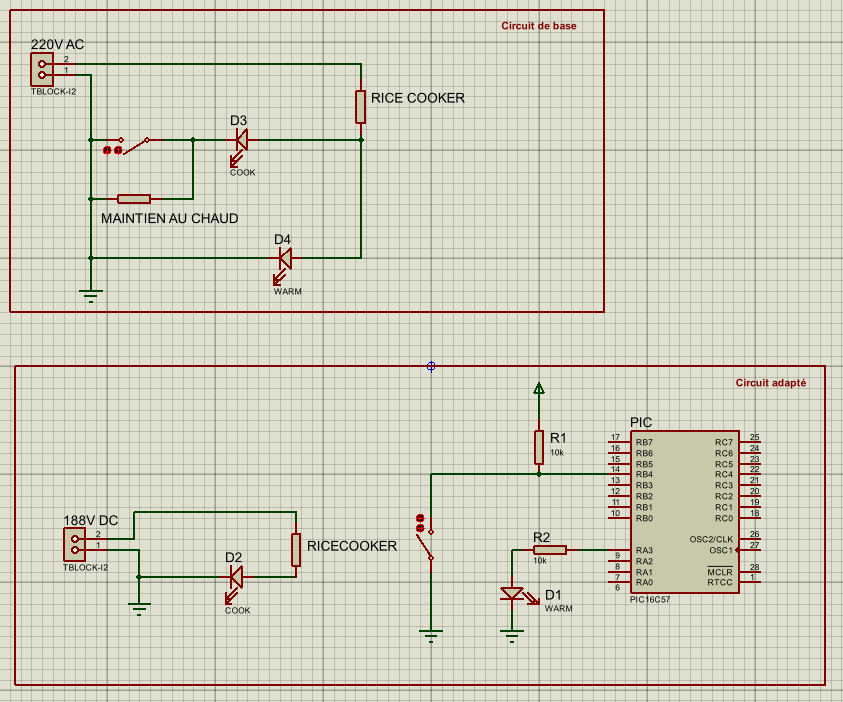
\includegraphics[width=0.8\linewidth]{images/Partie Rice cooker/28_Schéma contact rice cooker.png}
    \caption{Schéma Proteus de l'adaptation du capteur de température du Rice cooker.}
\end{figure}

\begin{decisionbox}[Décision : Rice-Cooker]
\textbf{Topologie :} Hacheur Dual Boost en T pour $450 \, \text{W}$ ($50 \to 188 \, \text{V}$). \\
\textbf{Pourquoi :} Bon compromis entre réduction de l'ondulation et coût composant par rapport à la version entrelacée. \\
\textbf{Impact système :} Diminution des pertes thermiques grâce aux rapports cycliques fragmentés ($\alpha = 0.37$) et préservation de la batterie via le maintien de conduction continue.
\end{decisionbox}

    \section{Lumières}
        \subsection{Solution technique}

L'objectif de cette section du projet est d'assurer l'alimentation de la partie éclairage du système, nous avions le choix entre un système alimenté sous 24~V ou 12~V. Nous avons opté pour un système de 24~V car ce choix présente trois avantages majeurs~:

\begin{itemize}
    \item \textbf{Moins de chauffe~:} Le courant étant divisé par deux, les pertes thermiques dans le cuivre sont divisées par quatre.
    \item \textbf{Meilleure stabilité~:} La chute de tension dans les pistes est réduite, garantissant un éclairage uniforme.
    \item \textbf{Standard industriel~:} Le 24~V est la tension de référence pour l'éclairage LED, facilitant le choix des composants.
\end{itemize}

Notre système est composé de 4 ampoules nécessitant une tension de 24~V. Nous devons donc abaisser la tension du bus principal de 48~V vers le 24~V.

Pour répondre à ce besoin, la solution technique retenue s'articule autour d'un convertisseur DC/DC 48~V/24~V. L'enjeu principal ici est de fournir une puissance suffisante et une tension de sortie parfaitement stable pour éviter tout effet de scintillement sur les luminaires. Un réseau de filtrage autour du convertisseur a été mis en place pour lisser la tension et absorber les appels de courant, tout en respectant les contraintes d'encombrement de la carte.

        \subsection{Dimensionnement des composants}

Le choix du convertisseur a été directement dicté par le bilan de puissance de l'éclairage~:

\begin{itemize}
    \item \textbf{Bilan de puissance et choix du convertisseur~:} Notre maison est constituée de 4 ampoules de 5~W chacune, ce qui représente une consommation totale de 20~W en régime établi. Pour garantir la fiabilité du système à long terme et un bon comportement thermique, nous avons opté pour un convertisseur DC/DC 48/24~V de 30~W. Cette marge de sécurité nous assure que le composant ne fonctionnera pas à sa limite maximale, évitant ainsi la surchauffe et prolongeant sa durée de vie.
    \item \textbf{Le filtrage~:} Pour la conception de l'étage de filtrage du convertisseur, nous nous sommes appuyés rigoureusement sur le schéma de filtrage fourni par le constructeur dans la datasheet~:
\end{itemize}

\begin{figure}[H]
    \centering
    
\includegraphics[width=0.8\linewidth]{images/Partie luminaires/01_Schéma filtre CEM.png}
    \caption{Schéma extrait de la datasheet du filtre CEM autour du convertisseur pour les luminaires.}
\end{figure}

Cependant, une adaptation majeure a été réalisée~: la suppression de l'inductance de mode commun en entrée. Bien que recommandée pour des environnements extrêmement pollués ou pour des équipements de communication très sensibles, cette bobine a été jugée superflue dans notre cas. Nos charges (des luminaires LED) sont intrinsèquement peu sensibles au bruit de mode commun. S'en affranchir nous a permis d'optimiser l'encombrement du PCB et de réduire les coûts, tout en maintenant un niveau de filtrage largement suffisant pour notre application.

Bien que l'inductance ait été retirée, le choix des condensateurs a été fait de manière stratégique en combinant deux technologies différentes pour couvrir tout le spectre des perturbations~:

\begin{itemize}
    \item \textbf{Condensateurs électrolytiques (Stockage d'énergie)~:} Placés en entrée, ils possèdent une forte capacité. Leur rôle est d'agir comme un réservoir "lent" mais massif. Ils encaissent les appels de courant importants (lors de l'allumage simultané des 4 ampoules) pour éviter que le bus 48~V ne s'effondre.
    \item \textbf{Condensateurs céramiques CMS - type X7R (Filtrage Haute Fréquence)~:} Utilisés pour le découplage au plus près des broches, leur très faible résistance série (ESR) leur permet de réagir instantanément. Ils sont indispensables pour "court-circuiter" vers la masse les parasites haute fréquence générés par le découpage interne du convertisseur, garantissant ainsi un 24~V parfaitement lisse. Le diélectrique X7R a été privilégié pour sa très bonne stabilité face aux variations de température induites par la puissance de la carte.
\end{itemize}

\begin{tableau}[H]
    \small
    \centering
    \begin{tabular}{|p{3cm}|p{3.5cm}|p{4.5cm}|p{4cm}|}
    \hline
    \textbf{Composant} & \textbf{Référence} & \textbf{Caractéristiques Clés} & \textbf{Rôle} \\
    \hline
    \textbf{Convertisseur} & \scriptsize REC30K4824SZ & DC/DC Isolé, 30~W, Entrée 48~V, Sortie 24~V & Abaisse la tension de 48~V à 24~V et isole galvaniquement la commande de la puissance. \\
    \hline
    \textbf{Inductance (L1)} & \scriptsize CLF7045T-100M-D & 10~$\mu$H, CMS (haute puissance/blindée) & Forme un filtre LC d'entrée avec les condensateurs pour bloquer les parasites de découpage. \\
    \hline
    \textbf{Capacité (C2)} & \scriptsize A786MW227M1HLAS011 & Forte capacité (220~$\mu$F typique), Électrolytique / Polymère & Réservoir d'énergie : absorbe les gros appels de courant à l'allumage des luminaires. \\
    \hline
    \textbf{Capacité (C3)} & \scriptsize GRM32EC72A106KE05K & 10~$\mu$F, Céramique CMS (X7R), Boîtier 1210 & Découplage d'entrée : filtre les parasites hautes fréquences (faible ESR). \\
    \hline
    \textbf{Capacités (C1, C4)} & \scriptsize C1812C472KDRACTU & 4,7~nF, Céramique Haute Tension (ex: 1~kV/2~kV) & Condensateurs "Y" : créent un chemin de retour pour le bruit de mode commun sans casser l'isolation. \\
    \hline
    \textbf{Capacité (C5)} & \scriptsize GRM32EC72A106KE05K & 10~$\mu$F, Céramique CMS (X7R), Boîtier 1210 & Lissage de sortie : stabilise la tension 24~V pour éviter le scintillement des LED. \\
    \hline
    \end{tabular}
    \caption{Choix des composants pour la partie Lumières.}
\end{tableau}

        \subsection{Schéma détaillé et PCB}

Nous avons le schéma final suivant~:

\begin{figure}[H]
    \centering
    \begin{subfigure}[b]{0.48\textwidth}
        \centering
        
\includegraphics[width=\linewidth]{images/Partie luminaires/02_Schéma proteus.pdf}
        \caption{Filtre et convertisseur (Proteus).}
    \end{subfigure}
    \hfill
    \begin{subfigure}[b]{0.48\textwidth}
        \centering
        
\includegraphics[width=\linewidth]{images/Partie luminaires/03_Routage du filtre du convertisseur pour les luminaires.png}
        \caption{Routage Top/Bottom.}
    \end{subfigure}
    \caption{Conception Carte Lumière.}
\end{figure}
\textbf{Bilan quantitatif :} La compacité de la carte de filtrage assure une stabilité à \SI{24}{\volt} tout en respectant l'espacement d'isolation.

\begin{decisionbox}[Décision : Éclairage]
\textbf{Topologie :} Abaissement $48 \, \text{V} \to 24 \, \text{V}$. \\
\textbf{Pourquoi :} L'utilisation du $24 \, \text{V}$ standard industriel permet de diviser par deux le courant, minimisant l'échauffement des fils et composants par rapport au $12 \, \text{V}$. \\
\textbf{Impact système :} Gains de stabilité sur l'éclairage (réduction du scintillement) et harmonisation globale des tensions domotiques.
\end{decisionbox}

    \section{USB-C}
        \subsection{Solution technique}

\subsubsection*{1.1 Choix de la topologie~: Le Convertisseur Buck Synchrone}

Pour fournir les 100~W demandés par le port USB-C, nous avons choisi d'utiliser un Hacheur abaisseur (Buck) Synchrone. Ce choix s'inspire directement des principes vus au premier semestre dans le module ENPU2. Même si nous n'avons pas étudié ce montage exact en cours, la théorie nous a donné les bases pour comprendre et utiliser cette architecture pour notre projet.

\begin{itemize}
    \item \textbf{Justification de l'abaisseur~:} Il permet de convertir efficacement la tension du bus batterie 48~V vers la tension cible stricte de 20~V.
    \item \textbf{Justification du Synchrone~:} Pour délivrer un courant de 5~A, l'utilisation d'une architecture asynchrone classique (avec une diode de roue libre) engendrerait des pertes thermiques importantes. Le remplacement de cette diode par un second transistor MOSFET contrôlé activement permet de réduire la chute de tension, d'augmenter le rendement global de la carte et de limiter l'échauffement thermique. C'est un point critique pour une carte compacte délivrant 100~W.
\end{itemize}

\subsubsection*{1.2 Le composant central~: Le contrôleur LM5116}

\paragraph{1.2.1 Le rôle du contrôleur~: Le Cerveau du système}
Pour bien comprendre le fonctionnement de notre convertisseur, il faut séparer la carte en deux parties distinctes : la puissance (les muscles) et la commande (le cerveau).

\begin{itemize}
    \item \textbf{Les Muscles (Les transistors MOSFET)~:} Ce sont eux qui encaissent la forte énergie de la batterie et agissent comme des interrupteurs ultra-rapides pour "hacher" la tension et la rabaisser à 20~V. Cependant, ces composants sont incapables de réfléchir : ils ne savent ni quand s'allumer, ni quand s'éteindre.
    \item \textbf{Le Cerveau (Le Contrôleur)~:} C'est la puce intelligente de notre carte. Son rôle est de surveiller en permanence ce qui se passe à la sortie du port USB-C. Si la tension chute brutalement, le contrôleur le détecte instantanément. Il envoie alors un signal aux muscles pour leur dire de s'ouvrir un peu plus longtemps afin de compenser. Il ajuste ce rythme des centaines de milliers de fois par seconde ! C'est ce pilotage qui garantit que l'utilisateur aura toujours un 20~V parfait et sécurisé, quoi qu'il arrive.
\end{itemize}


\paragraph{1.2.2 Tableau comparatif~: LM5116 vs LM5117}
Pour jouer ce rôle crucial, nous avons comparé deux composants performants : le LM5116 et le LM5117. Voici le bilan de notre étude :

\begin{tableau}[htbp]
    \centering
    \begin{tabular}{|p{4cm}|p{2cm}|p{2cm}|p{6cm}|}
    \hline
    \textbf{Caractéristique} & \textbf{LM5116} & \textbf{LM5117} & \textbf{Impact pour le projet} \\
    \hline
    \textbf{Tension d'entrée Max} & 100~V & 65~V & Sécurité : Le LM5116 offre une marge bien plus grande face aux pics de tension de la batterie. \\
    \hline
    \textbf{Mesure de courant (Current Monitor)} & Non & Oui & Le LM5117 permet de surveiller le courant en temps réel, mais ce n'était pas une priorité pour nous. \\
    \hline
    \textbf{Tension de référence} & 1,215~V & 0,8~V & Cela change simplement la valeur des résistances pour régler le 20~V en sortie. \\
    \hline
    \end{tabular}
    \caption{Comparatif LM5116 et LM5117.}
\end{tableau}

\paragraph{1.2.3 Pourquoi avoir choisi le LM5116~?}
Le facteur décisif de notre choix a été la sécurité et la robustesse. Notre batterie pouvant monter jusqu'à 56~V, le LM5117 (limité à 65~V) offrait une marge de sécurité trop faible et risquait de griller en cas de problème sur le bus. En choisissant le LM5116, qui accepte une tension d'entrée allant jusqu'à 100~V, nous protégeons efficacement notre carte contre les surtensions brutales.

Outre cet avantage décisif sur la tension, le LM5116 regroupe toutes les caractéristiques indispensables à notre projet~:

\begin{itemize}
    \item \textbf{Un contrôle avancé (Emulated Current Mode)~:} Cette méthode de régulation assure une grande stabilité de la tension de sortie à 20~V, ce qui est vital pour compenser instantanément les fortes variations de courant demandées par un appareil branché en USB-C.
    \item \textbf{Un pilotage intégré (Drivers)~:} La puce intègre nativement les "drivers" (amplificateurs de commande) nécessaires pour piloter directement les deux gros MOSFETs de puissance. Cela nous évite d'ajouter des composants supplémentaires et optimise considérablement l'encombrement sur le circuit imprimé.
    \item \textbf{Un démarrage progressif (Soft-start)~:} Pour un convertisseur délivrant 100~W, une mise sous tension brutale créerait un pic de courant destructeur. La puce intègre une fonction permettant de faire monter la tension de sortie en douceur jusqu'à 20~V, garantissant un allumage sécurisé pour nos composants.
\end{itemize}

\begin{figure}[H]
    \centering
    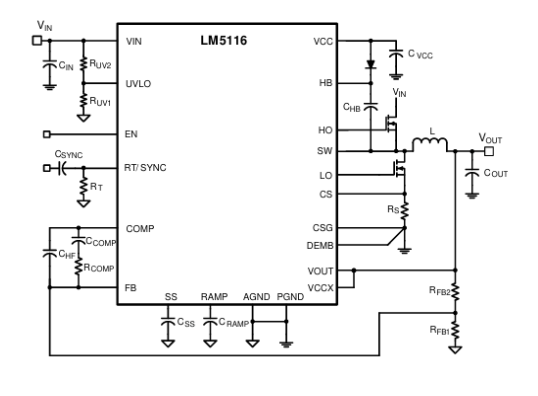
\includegraphics[width=0.8\linewidth]{images/Partie USB-C/01_Schéma d_application typique du LM5116 illustrant le pilotage intégré des MOSFETs de puissance (Source _ Datasheet Texas Instruments).png}
    \caption{Schéma d'application typique du LM5116 illustrant le pilotage intégré des MOSFETs de puissance (Source~: Datasheet Texas Instruments).}
\end{figure}

\subsubsection*{1.3 Intégration dans l'architecture globale}
Le choix de réaliser la fonction USB-C sur une carte PCB unique et détaillée permet d'intégrer ce module de haute puissance au sein d'une architecture globale modulaire. Cette carte est alimentée en parallèle sur le bus principal de 48~V, ce qui assure une distribution d'énergie indépendante de celle des autres modules tout en partageant une masse commune pour garantir la stabilité des signaux. Avec une puissance de sortie de 100~W, ce PCB dédié joue un rôle crucial dans la gestion thermique du système~: il permet d'isoler la zone de forte dissipation de chaleur, protégeant ainsi l'électronique de contrôle plus sensible située sur les autres cartes du projet.

        \subsection{Dimensionnement des composants}

Pour garantir les performances de notre carte (20~V pour 5~A), nous avons débuté par une étude théorique des composants de puissance en nous inspirant des concepts vus dans le module ENPU2. Ces premiers calculs ont ensuite été validés par une simulation sur modèle idéal. Pour cette étape, nous nous sommes basés sur les paramètres nominaux suivants~: une tension d'entrée de 48~V et une fréquence de découpage fixée à 400~kHz.

\subsubsection*{2.1. Calculs théoriques du convertisseur}

\paragraph{2.1.1. Le Rapport Cyclique ($\alpha$)}
Le rapport cyclique définit le temps de conduction nécessaire pour rabaisser la tension d'entrée. En négligeant les pertes du système idéal, il se calcule ainsi~:

$$ \alpha = \frac{V_{\text{out}}}{V_{\text{in}}} = \frac{20}{48} = 0,416 $$

Soit un rapport cyclique de 41,6\,\%.

\paragraph{2.1.2. Dimensionnement de l'Inductance ($L$)}
Pour assurer un bon compromis entre la taille du composant et la stabilité, nous avons fixé l'ondulation de courant ($\Delta I_L$) à 1~A (soit 20\,\% du courant nominal de 5~A). Le courant oscille donc entre $I_{L\text{min}} = 4,5~\text{A}$ et $I_{L\text{max}} = 5,5~\text{A}$. La valeur de la bobine s'obtient avec la formule suivante~:

$$ L = \frac{\alpha \cdot (1-\alpha) \cdot V_{\text{out}}}{\Delta I_L \cdot F} = \frac{0,416 \cdot (1-0,416) \cdot 48}{1 \cdot 400000} \approx 29,15~\mu\text{H} $$
% Note: L'équation du rapport utilise V_in dans le numérateur au lieu de V_out ? L'équation originale est L = (\alpha * (1-\alpha) * Vin)/(\Delta I * F). Le calcul de 29,15 µH découle de 0,416 * 0,584 * 48 / 400000 = 29,149 µH. C'est exact.

On choisit la valeur normalisée $L = 30~\mu\text{H}$.

L'énergie maximale stockée dans cette inductance est d'environ~:

$$ E_L = \frac{1}{2} L I_{L\text{max}}^2 = \frac{1}{2} \cdot 30\cdot 10^{-6} \cdot 5,5^2 \approx 440,9~\mu\text{J} $$

\paragraph{2.1.3. Dimensionnement des Condensateurs de filtrage ($C_s$ et $C_e$)}
Pour garantir la qualité de la tension et protéger nos composants, nous avons imposé des contraintes d'ondulation très strictes~:

\begin{itemize}
    \item \textbf{Condensateur de sortie ($C_s$)~:} Pour une ondulation maximale autorisée de 1\,\% (soit une variation de 0,2~V sur les 20~V attendus), le calcul théorique donne~: \\
    $$ C_S = \frac{\alpha \cdot (V_{\text{in}} - V_{\text{out}})}{8 \cdot L \cdot F^2 \cdot \Delta V_{\text{out}}} = \frac{0,416 \cdot (48 - 20)}{8 \cdot 29,15 \cdot 10^{-6} \cdot (400000)^2 \cdot 0,2} = 1,56~\mu\text{F} $$ \\
    On choisit la valeur normalisée $C_s = 1,6~\mu\text{F}$.
    \item \textbf{Condensateur d'entrée ($C_e$)~:} Pour limiter les perturbations sur le bus batterie avec une ondulation maximale tolérée de 0,5~V, le calcul donne~: \\
    $$ C_e = \frac{I_s \cdot \alpha \cdot (1 - \alpha)}{F \cdot \Delta V_{\text{in}}} = \frac{5 \cdot 0,416 \cdot (1-0,416)}{400000 \cdot 0,5} = 6,07~\mu\text{F} $$ \\
    On choisit la valeur normalisée $C_e = 6,2~\mu\text{F}$.
\end{itemize}

\subsubsection*{2.2. Validation du modèle théorique par simulation (PSIM)}

Afin de vérifier la justesse de nos calculs mathématiques avant de passer à l'implémentation réelle, nous avons modélisé cette architecture de puissance sur le logiciel PSIM.

\begin{figure}[H]
    \centering
    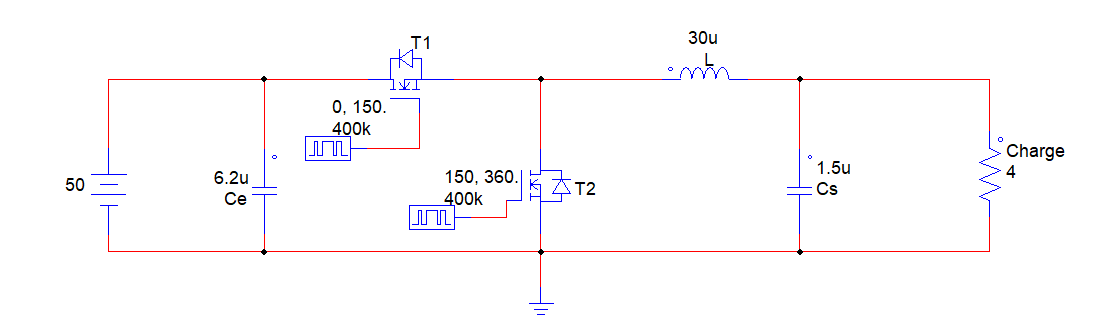
\includegraphics[width=0.8\linewidth]{images/Partie USB-C/02_Schéma de simulation PSIM du convertisseur Buck Synchrone avec les valeurs théoriques calculées.png}
    \caption{Schéma de simulation PSIM du convertisseur Buck Synchrone avec les valeurs théoriques calculées.}
\end{figure}

Ce schéma de principe présente notre source de 48~V (dimensionnée avec une valeur maximale de 50~V), nos composants passifs dimensionnés et une charge résistive de 4 ohms simulant un appel de courant continu de 5~A. Le pilotage des transistors (T1 et T2) est assuré par des blocs de commande idéaux configurés à 400~kHz respectant notre rapport cyclique de 0,416.

\textbf{Analyse des résultats~:}

\begin{figure}[H]
    \centering
    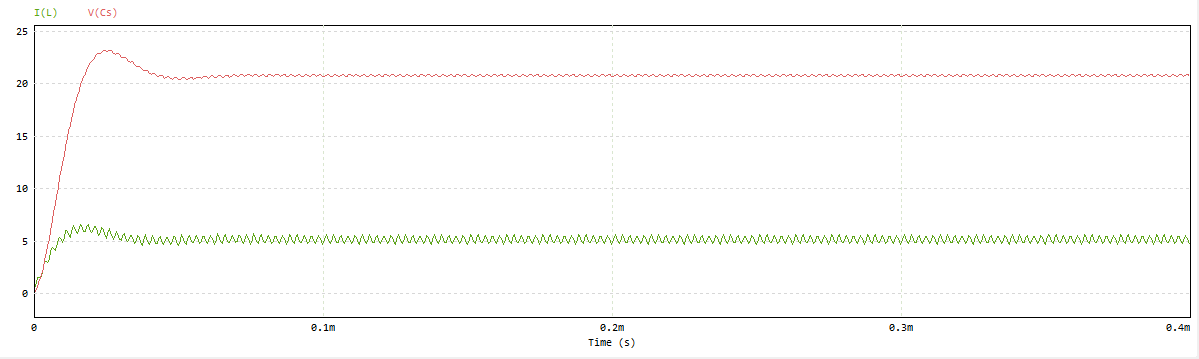
\includegraphics[width=0.8\linewidth]{images/Partie USB-C/03_Relevés de la simulation théorique (Tension de sortie V(Cs) en rouge, Courant d_inductance I(L) en vert).png}
    \caption{Relevés de la simulation théorique (Tension de sortie V(Cs) en rouge, Courant d'inductance I(L) en vert).}
\end{figure}

Les courbes générées par la simulation confirment notre dimensionnement théorique en régime permanent~:
\begin{itemize}
    \item \textbf{La tension de sortie (en rouge)~:} Elle se stabilise bien autour de la valeur cible de 20~V.
    \item \textbf{Le courant dans l'inductance (en vert)~:} Le courant moyen fourni à la charge est bien de 5~A. L'ondulation forme les dents de scie caractéristiques, avec une amplitude d'environ 1~A, respectant ainsi nos calculs.
\end{itemize}

\textbf{Les limites de ce modèle idéal~:} Bien que ce schéma valide la théorie, il présente trois défauts majeurs qui nous empêchent de l'utiliser tel quel pour notre PCB réel~:
\begin{itemize}
    \item \textbf{Un démarrage brutal (Absence de Soft-Start)~:} Comme on le voit au tout début de la courbe rouge, la tension fait un pic (dépassement) à près de 23~V avant de se stabiliser. Sur un vrai port USB-C, cette surtension transitoire pourrait détruire l'appareil connecté.
    \item \textbf{Une commande en boucle ouverte~:} Ici, le rapport cyclique est fixe. Si l'utilisateur débranche son appareil (changement de la charge), la tension ne restera pas à 20~V. Il nous manque un cerveau pour réguler la sortie.
    \item \textbf{L'absence de contraintes physiques~:} Ce modèle ignore les temps morts (Dead-Time) indispensables pour éviter les courts-circuits entre les vrais MOSFETs, ainsi que les éléments parasites (inductances des câbles, résistances séries).
\end{itemize}

C'est pourquoi nous avons dû faire évoluer cette simulation vers un modèle réaliste en boucle fermée.

\subsubsection*{2.3. Transition vers une simulation réaliste}
La première simulation nous a permis de valider la chaîne d'énergie idéale. Cependant, un convertisseur réel ne fonctionne jamais à rapport cyclique fixe, et les composants parfaits n'existent pas. Pour nous rapprocher du comportement exact de notre futur PCB et de notre contrôleur LM5116, nous avons fait évoluer le modèle PSIM vers une architecture en boucle fermée intégrant les contraintes physiques réelles.

\begin{figure}[H]
    \centering
    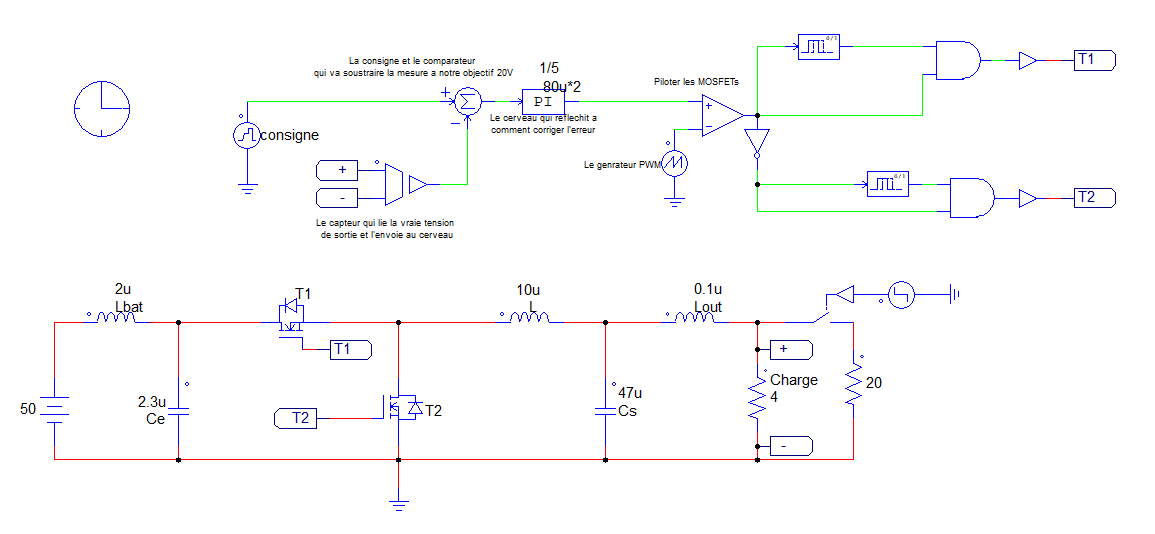
\includegraphics[width=0.8\linewidth]{images/Partie USB-C/04_Modèle PSIM réaliste intégrant l_asservissement PI, les temps morts et les éléments parasites.png}
    \caption{Modèle PSIM réaliste intégrant l'asservissement PI, les temps morts et les éléments parasites.}
\end{figure}

Ce schéma de niveau avancé introduit des modifications majeures et justifiées :

\paragraph{2.3.1. L'intégration de la régulation (Le Cerveau et le PWM)}
Dans la réalité, la charge branchée sur un port USB-C varie constamment (l'appareil tire plus ou moins de courant selon sa batterie). Pour maintenir un 20~V strict, nous avons remplacé la commande ouverte par une véritable boucle de régulation~:
\begin{itemize}
    \item \textbf{La mesure~:} Un capteur lit la tension de sortie réelle et la compare à notre consigne stricte de 20~V.
    \item \textbf{Le Régulateur PI (Proportionnel Intégral)~:} L'erreur calculée est envoyée à ce correcteur. Les valeurs (Gain de 1/5 et Constante de temps de 160~$\mu$s) ont été ajustées empiriquement en simulation. L'objectif était de trouver le compromis parfait : le système doit réagir très vite à une variation de charge, mais sans créer de dépassement dangereux qui ferait monter la tension au-delà de 20~V et grillerait l'appareil branché.
    \item \textbf{Le générateur PWM~:} La sortie de ce régulateur dicte au générateur PWM d'augmenter ou de réduire automatiquement la largeur des impulsions envoyées aux MOSFETs.
\end{itemize}

\paragraph{2.3.2. Sécurité : Le choix du Temps Mort (Dead-Time)}
Sur un convertisseur Buck Synchrone, il est absolument vital que le transistor T1 (High-Side) et le transistor T2 (Low-Side) ne soient jamais fermés en même temps. Si cela arrivait, cela créerait un court-circuit direct entre le 48~V et la masse (phénomène de shoot-through), ce qui détruirait la carte instantanément.

\textbf{Justification des 200~ns~:} La datasheet de notre contrôleur LM5116 indique qu'il intègre nativement un temps mort adaptatif (autour de 150~ns). Dans notre simulation PSIM, nous avons modélisé cette sécurité en imposant des blocs de retard de 200~ns. Cette légère marge supplémentaire (50~ns) permet de prendre en compte le temps de commutation réel (Turn-ON et Turn-OFF) des MOSFETs de puissance physiques que nous allons souder sur la carte.

\paragraph{2.3.3. Modélisation des contraintes physiques et choix des composants}
\begin{itemize}
    \item \textbf{Les inductances parasites ($L_{\text{bat}}$ et $L_{\text{out}}$)~:} Nous avons ajouté une $L_{\text{bat}}$ de 2~$\mu$H et une $L_{\text{out}}$ de 0,1~$\mu$H. Elles simulent l'impédance inévitable des câbles physiques qui relieront la batterie à notre PCB, et notre PCB au connecteur USB-C.
    \item \textbf{La résistance de pré-charge ($R = 20~\Omega$)~:} Placée en parallèle de la sortie, elle impose un courant d'entretien minimal. Sans elle, si aucun appareil n'est branché sur l'USB-C, le courant chuterait à zéro et le convertisseur passerait en conduction discontinue, ce qui rendrait la boucle de régulation instable.
    \item \textbf{L'optimisation du filtre LC ($L$ passe à 10~$\mu$H, $C_s$ passe à 47~$\mu$F)~:} L'inductance théorique de 29~$\mu$H calculée précédemment serait physiquement très volumineuse et chère pour supporter 5~A. Nous l'avons remplacée par une valeur standardisée plus faible de 10~$\mu$H. Cela permet d'utiliser un composant plus petit, moins cher, et qui offre une réponse dynamique plus rapide.
    \item \textbf{La compensation ($C_s$ et $C_e$)~:} Réduire la bobine augmente inévitablement l'ondulation du courant. Pour compenser ce phénomène et garder une tension de sortie parfaitement lisse à 20~V, nous avons dû augmenter considérablement la capacité du condensateur de sortie, qui passe à un standard de 47~$\mu$F. Le condensateur d'entrée ($C_e$) a également été ajusté à 2,3~$\mu$F pour absorber les appels de courant modifiés par cette nouvelle bobine.
\end{itemize}

\textbf{Validation des performances du modèle réaliste} \\
Pour vérifier l'efficacité de nos modifications et du régulateur PI, nous avons effectué des relevés sur ce nouveau modèle en boucle fermée.

\begin{figure}[H]
    \centering
    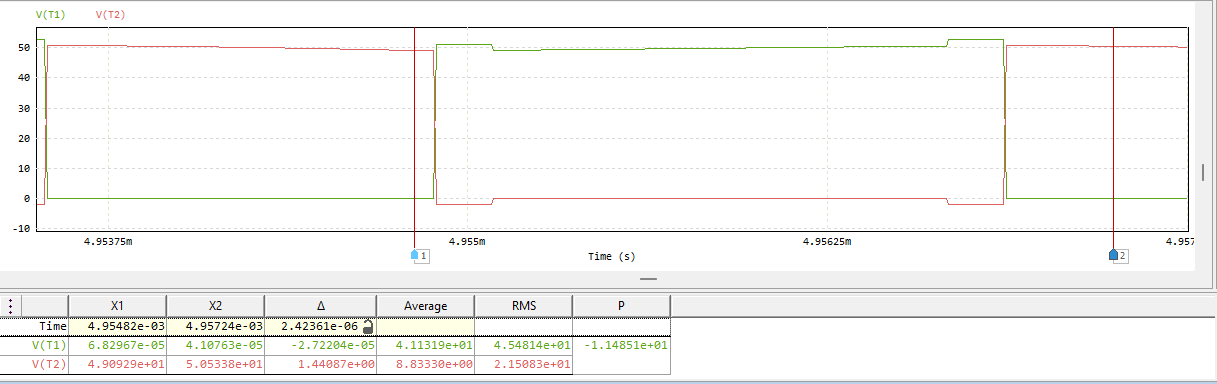
\includegraphics[width=0.8\linewidth]{images/Partie USB-C/05_Zoom sur les signaux de commande des MOSFETs illustrant le Temps Mort (Dead-Time)..png}
    \caption{Zoom sur les signaux de commande des MOSFETs illustrant le Temps Mort (Dead-Time).}
\end{figure}

\textbf{Analyse de la sécurité (Temps Mort)~:} La figure précédente montre les signaux de grille du transistor High-Side V(T1) en vert et Low-Side V(T2) en rouge. L'observation minutieuse des fronts de commutation (lorsqu'un signal descend et que l'autre monte) montre clairement un espacement où les deux signaux sont à zéro simultanément. Ce délai valide le paramétrage de notre temps mort de 200~ns, garantissant qu'aucun court-circuit ne se produira dans notre étage de puissance.

\begin{figure}[H]
    \centering
    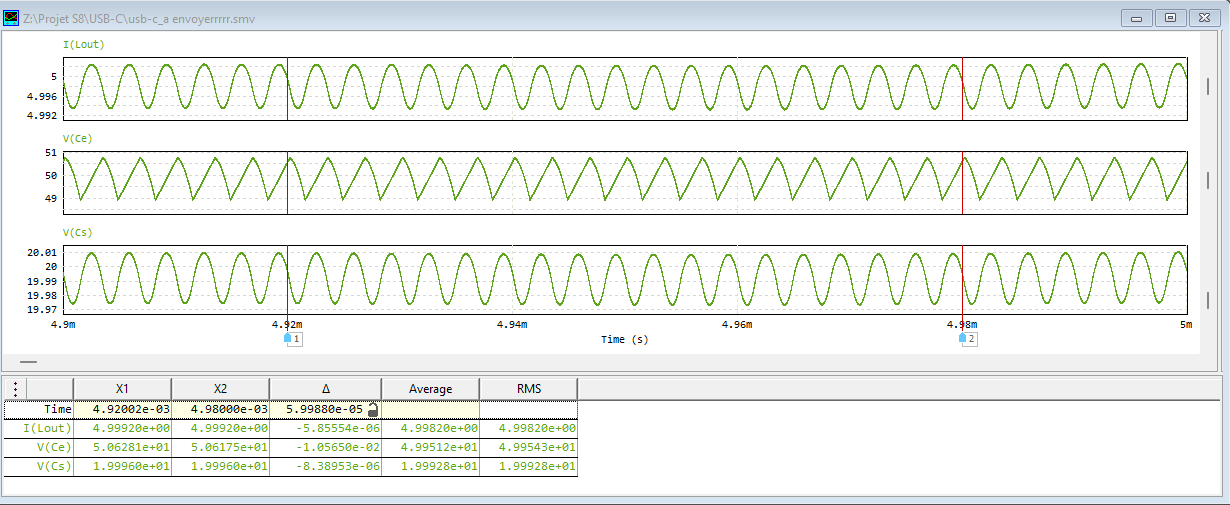
\includegraphics[width=0.8\linewidth]{images/Partie USB-C/06_Relevés en régime permanent du convertisseur avec boucle de régulation (Courant d_inductance, Tension d_entrée et Tension de sortie).png}
    \caption{Relevés en régime permanent du convertisseur avec boucle de régulation (Courant d'inductance, Tension d'entrée et Tension de sortie).}
\end{figure}

\textbf{Analyse de la régulation et du filtrage~:}

La figure illustre le comportement du système en régime établi (autour de $t = 5~\text{ms}$) et valide nos choix de condensateurs :
\begin{itemize}
    \item \textbf{La tension de sortie V($C_s$)~:} Le tableau de mesures indique une moyenne de 19,99~V. Le régulateur PI remplit parfaitement son rôle d'asservissement en effaçant l'erreur statique. Grâce à notre capacité $C_s$ de 47~$\mu$F, l'ondulation est extrêmement faible (quelques millivolts), garantissant un signal pur pour le port USB-C.
    \item \textbf{La tension d'entrée V($C_e$)~:} La moyenne est bien stabilisée autour de 50~V (bus 48~V chargé). L'ondulation visible prouve que notre condensateur d'entrée de 2,3~$\mu$F joue bien son rôle d'amortisseur pour éviter de polluer le reste du système global avec le découpage.
    \item \textbf{Le courant d'inductance I($L_{\text{out}}$)~:} La valeur moyenne mesurée est de 4,99~A. Le système délivre la puissance maximale attendue, avec une ondulation triangulaire stable malgré la réduction de l'inductance à 10~$\mu$H.
\end{itemize}

Cette simulation avancée valide définitivement l'architecture fonctionnelle de notre carte.

        \subsection{Étude Industrielle et Choix des Composants (TI Webench)}

Si la simulation PSIM a validé notre architecture, elle reste théorique. Pour passer à la réalisation du PCB, nous avons utilisé l'outil TI Webench Power Designer. Contrairement à PSIM, Webench intègre les modèles réels des constructeurs et prend en compte les caractéristiques complexes des broches du LM5116.

\subsubsection*{3.1. Du modèle idéal au schéma réel}
Le passage de la simulation PSIM à la réalité industrielle avec l'outil TI Webench nous confronte à la complexité réelle du contrôleur LM5116. Cette puce possède 20 broches qui nécessitent chacune un réseau précis de composants passifs périphériques pour assurer toutes ses fonctions de sécurité, de pilotage et d'asservissement. \\
Nous avons configuré Webench avec nos contraintes ($V_{\text{in}} = 42\text{V}/56\text{V}$, $V_{\text{out}} = 20\text{V}$, $I_{\text{out}} = 5\text{A}$) afin d'obtenir une structure optimisée.

\begin{figure}[H]
    \centering
    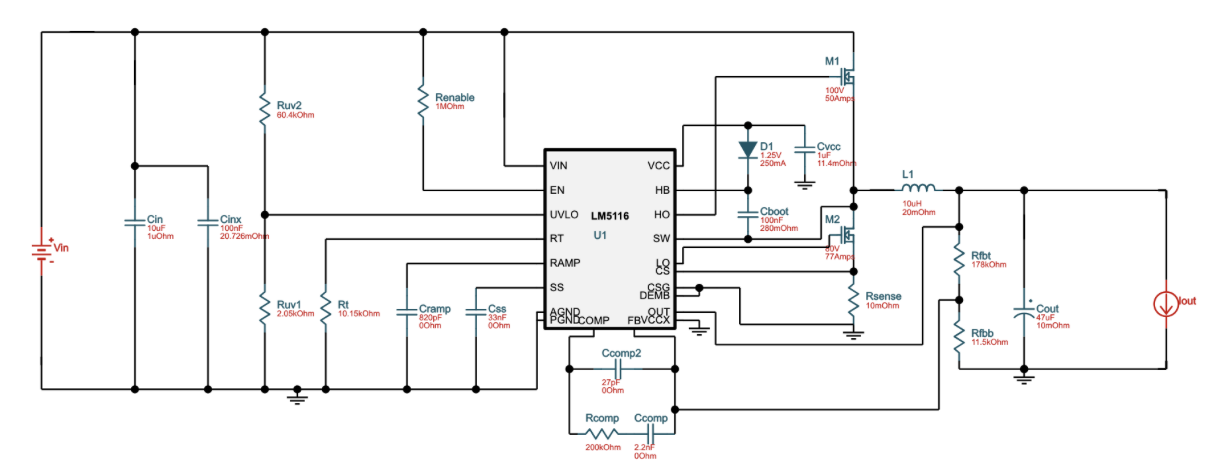
\includegraphics[width=0.8\linewidth]{images/Partie USB-C/07_Schéma Webench complet intégrant l_intégralité des composants passifs périphériques..png}
    \caption{Schéma Webench complet intégrant l'intégralité des composants passifs périphériques.}
\end{figure}

C’est sur la base de ce schéma que nous avons validé notre stratégie. Voici l'analyse détaillée des différents blocs fonctionnels de notre puce :

\paragraph{3.1.1. L'alimentation stratégique et la gestion des masses (Points critiques du PCB)}
\begin{itemize}
    \item \textbf{Le convertisseur 5V/12V externe~:} Par défaut, le LM5116 utilise son régulateur interne pour générer sa propre tension logique à partir du bus 48~V, ce qui engendre d'importantes pertes thermiques. Notre projet d'équipe disposant d'une source 5~V, nous avons pris la décision d'ajouter le convertisseur MPFN1-05S12AN (Farnell). Cela nous permet de désactiver le régulateur interne et d'alimenter directement la broche VCC avec un 12~V propre. Ce choix soulage la puce thermiquement et garantit des signaux de commande puissants. De plus, pour garantir la stabilité de cette alimentation et empêcher la propagation de bruit parasite vers notre contrôleur, nous avons complété ce module par un réseau de filtrage capacitif (condensateurs de découplage) en entrée et en sortie. La documentation technique du convertisseur Farnell ne spécifiant pas de valeurs exactes, nous avons dimensionné ces capacités à 10~$\mu$F en accord avec l'encadrement technique. Cette valeur standard de l'industrie est parfaitement adaptée pour lisser les ondulations de ce type de convertisseur compact.
\end{itemize}

\begin{figure}[H]
    \centering
    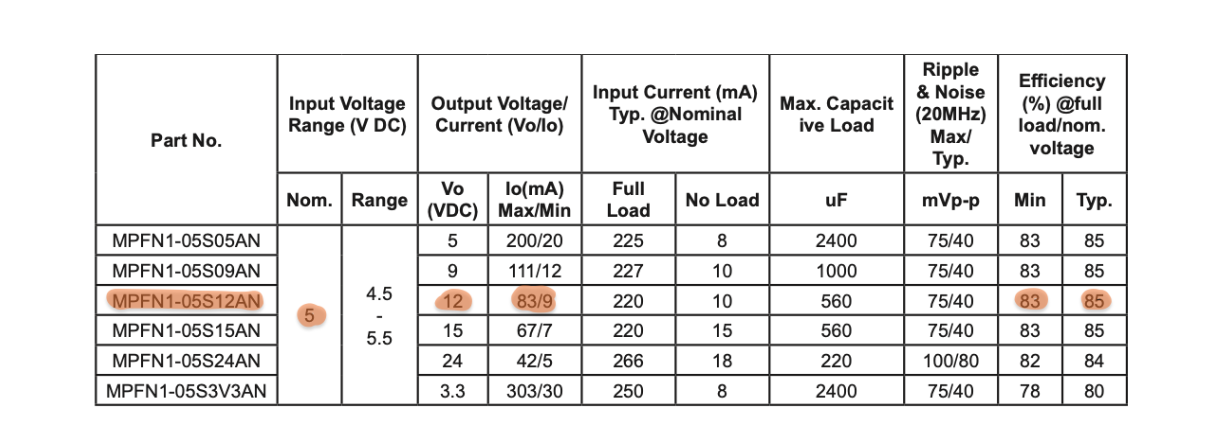
\includegraphics[width=0.8\linewidth]{images/Partie USB-C/08_Référence du convertisseur DC_DC 5V vers 12V (Farnell) utilisé pour l_alimentation logique..png}
    \caption{Référence du convertisseur DC/DC 5V vers 12V (Farnell) utilisé pour l'alimentation logique.}
\end{figure}

\begin{itemize}
    \item \textbf{La masse séparée (AGND vs PGND)~:} C’est un point stratégique de notre routage. La broche PGND (Masse Puissance) regroupe les retours de forts courants (très bruités). La broche AGND (Masse Analogique) est dédiée aux signaux de commande sensibles (FB, COMP, RAMP). En séparant physiquement AGND de PGND sur le circuit imprimé avec un point de liaison unique, nous protégeons le cerveau des parasites de puissance.
\end{itemize}

\paragraph{3.1.2. Le pilotage de la puissance (Les Drivers)}
\begin{itemize}
    \item \textbf{HO et LO (High / Low Output)~:} Ce sont les sorties de commande directes qui envoient les signaux PWM aux grilles de nos deux MOSFETs de puissance (M1 et M2).
    \item \textbf{Le circuit Bootstrap (Broche HB)~:} Composé de la diode D1 et du condensateur $C_{\text{boot}}$ (100~nF), ce circuit agit comme une mini-pompe de charge. Il est indispensable pour rendre passant le transistor High-Side (M1), dont la grille doit être portée à une tension localement supérieure à celle du bus 48~V.
\end{itemize}

\paragraph{3. La sécurité et le démarrage progressif}
\begin{itemize}
    \item \textbf{UVLO (Under-Voltage Lockout) et EN (Enable)~:} Ces broches sont reliées à un pont diviseur précis ($R_{\text{uv2}} = 60,4~\text{k}\Omega$ et $R_{\text{uv1}} = 2,05~\text{k}\Omega$). UVLO bloque le démarrage si la batterie est trop faible, évitant un comportement erratique, tandis qu'EN agit comme l'interrupteur logique ON/OFF de notre carte.
    \item \textbf{SS (Soft-Start)~:} Le condensateur $C_{ss}$ (33~nF) force la tension de sortie à monter doucement vers 20~V. Cela évite les arcs électriques et les pics de courant destructeurs lors du branchement d'un appareil déchargé sur le port USB-C.
\end{itemize}

\paragraph{4. La mesure et le Cerveau (La Régulation)}
\begin{itemize}
    \item \textbf{FB (Feedback)~:} C'est l'œil du contrôleur. Il reçoit une image réduite de la tension de sortie grâce au pont diviseur $R_{\text{fbt}}$ (178~k$\Omega$) et $R_{\text{fbb}}$ (11,5~k$\Omega$) pour vérifier que la sortie est bien maintenue à 20~V.
    \item \textbf{COMP (Compensation)~:} C’est la transposition physique de notre régulateur PI vu sous PSIM. Le réseau composé de $R_{\text{comp}}$, $C_{\text{comp}}$ et $C_{\text{comp2}}$ ajuste la réponse dynamique pour garantir que le système réagit vite aux variations de charge sans jamais osciller.
    \item \textbf{CS et CSG (Current Sense)~:} Ces broches surveillent le courant de sortie en mesurant la chute de tension aux bornes d'une très faible résistance de shunt ($R_{\text{sense}} = 10~\text{m}\Omega$). Cela permet de couper instantanément le système en cas de court-circuit.
\end{itemize}

\paragraph{5. Les réglages internes}
\begin{itemize}
    \item \textbf{RT~:} Cette broche fixe l'horloge interne de la puce. La résistance $R_t$ (10,15~k$\Omega$) est précisément dimensionnée pour imposer notre fréquence de découpage de 400~kHz.
    \item \textbf{RAMP~:} Le condensateur $C_{\text{ramp}}$ génère le signal en dent de scie nécessaire à l'architecture de contrôle avancée "Emulated Current Mode" du LM5116.
\end{itemize}

\subsubsection*{3.2. Choix des composants de Puissance}
Maintenant que la logique de commande est validée et sécurisée, il est crucial de dimensionner la chaîne de puissance capable d'encaisser les 100~W (20~V / 5~A) sans surchauffe. Webench nous a permis de sélectionner les références industrielles exactes en optimisant les caractéristiques critiques ($R_{DS(on)}$, ESR, Saturation) :

\begin{tableau}[H]
    \centering
    \scriptsize
    \begin{tabular}{|p{3cm}|>{\raggedright\arraybackslash}p{3cm}|p{3cm}|>{\raggedright\arraybackslash}p{5cm}|}
    \hline
    \textbf{Composant} & \textbf{Référence (Farnell)} & \textbf{Rôle Technique} & \textbf{Justification du Choix} \\
    \hline
    \textbf{MOSFET High-Side} & BSC220N20NSFDATMA1 & Interrupteur principal & Canal N acceptant jusqu'à 200~V et 52~A. Marge de sécurité face aux surtensions du bus 48~V. Très faible $R_{DS(on)}$ ($17,7~\text{m}\Omega$) pour limiter les pertes thermiques. \\
    \hline
    \textbf{MOSFET Low-Side} & BSC220N20NSFDATMA1 & Redressement synchrone & Choisi identique au High-Side pour simplifier la maintenance et l’assemblage de la carte. \\
    \hline
    \textbf{Inductance (L)} & SRP1265A-100M & Stockage d'énergie & Blindée et solide. Évite d'envoyer des ondes parasites au cerveau. Laisse passer les 5~A sans saturer. \\
    \hline
    \textbf{Condensateur de sortie} & 875075555002 & Filtrage de tension & Condensateur CMS de 47~$\mu$F. Tension de service de 25~V optimale pour sécuriser notre sortie stabilisée à 20~V, tout en conservant une taille compacte. \\
    \hline
    \textbf{Diode Bootstrap} & ES1PB-M3/84A & Alimentation Driver & Indispensable pour permettre au LM5116 de piloter le MOSFET du haut. \\
    \hline
    \end{tabular}
    \caption{Choix des composants de puissance (USB-C).}
\end{tableau}

\subsubsection*{3.3. Gestion Thermique : Calcul des pertes et Dissipation}
Avec une puissance de 100~W, la chaleur générée par les MOSFETs est un point critique. Nous avons réalisé un bilan thermique pour vérifier si les composants peuvent fonctionner sans risque de destruction.

\paragraph{3.3.1. Calcul des pertes de puissance ($P_d$)}
En nous basant sur les caractéristiques de la datasheet du MOSFET BSC220N20NSF (notamment les temps de commutation $t_r = 7~\text{ns}$ et $t_f = 10~\text{ns}$), nous avons calculé les pertes totales qui se divisent en deux catégories :

\textbf{Les pertes par conduction ($P_{\text{cond}}$)~:} Elles sont dues à la résistance interne du composant lorsqu'il est passant. La formule dépend du rapport cyclique, du courant de sortie et de la résistance du MOSFET~:
$$ P_{\text{cond}} = R_{DS(on)} \cdot I_{\text{out}}^2 \cdot \alpha $$
Avec nos valeurs : $R_{DS(on)} = 17,7~\text{m}\Omega$, $I_{\text{out}} = 5~\text{A}$, et $\alpha = 0,416$
$$ P_{\text{cond}} = 0,0177 \cdot 5^2 \cdot 0,416 \approx 0,184~\text{W} $$

\textbf{Les pertes par commutation ($P_{\text{sw}}$)~:} Elles se produisent à chaque fois que le transistor s'allume et s'éteint, créant un croisement entre la tension et le courant. La formule utilise les temps de montée ($t_r$) et de descente ($t_f$) donnés dans la datasheet du composant, ainsi que la fréquence de découpage ($F$)~:
$$ P_{\text{sw}} = \frac{1}{2} \cdot V_{\text{in}} \cdot I_{\text{out}} \cdot (t_r + t_f) \cdot F $$
Avec nos valeurs~:
$$ P_{\text{sw}} = \frac{1}{2} \cdot 48 \cdot 5 \cdot (7\cdot 10^{-9} + 10 \cdot 10^{-9}) \cdot 400000 \approx 0,816~\text{W} $$

\textbf{Puissance totale dissipée~:} Pour obtenir la chaleur totale générée par le composant, on additionne ces deux valeurs. En ajoutant une petite marge de sécurité pour les pertes secondaires (comme la charge de la grille), on obtient :
$$ P_{\text{tot}} = P_{\text{cond}} + P_{\text{sw}} \approx 0,184 + 0,816 \approx 1~\text{W} $$
Avec la marge de sécurité thermique appliquée (liée à l'augmentation de la résistance avec la chaleur), nous avons arrondi notre estimation de puissance maximale à dissiper à 1,16~W par MOSFET.

\paragraph{3.3.2. Détermination du besoin en refroidissement}
L'objectif est de maintenir la température de jonction du composant en dessous de $120~^\circ\text{C}$ pour garantir sa durée de vie.

Le calcul de la résistance thermique totale maximale autorisée ($R_{\text{thmax}}$) nous donne un besoin théorique : il nous faut un refroidissement total inférieur à $68~^\circ\text{C/W}$.

\paragraph{3.3.3. Choix de la solution technique : Dissipateurs CMS}
Initialement, nous avions envisagé d'utiliser uniquement de larges zones de cuivre sur le PCB pour dissiper la chaleur (offrant environ 40 à $50~^\circ\text{C/W}$). Cependant, pour garantir une sécurité industrielle maximale et répondre aux standards de robustesse, nous avons suivi les recommandations de l'encadrement en intégrant des dissipateurs thermiques CMS (type Heatsink soudable).

\begin{tableau}[H]
    \footnotesize
    \centering
    \begin{tabular}{|l|l|l|}
    \hline
    \textbf{Composant} & \textbf{Référence} & \textbf{Rôle} \\
    \hline
    Dissipateur thermique & 573300D00010G & Augmenter la surface d'échange thermique avec l'air. \\
    \hline
    \end{tabular}
\end{tableau}

\subsubsection*{3.4. Validation dynamique et temporelle (Simulations Webench)}
Pour nous assurer de la fiabilité de nos composants industriels, nous avons soumis notre modèle Webench à deux tests de simulation critiques~: le régime permanent (Steady State) et la réponse transitoire (Load Transient).

\textbf{1. Test de l'ondulation en régime permanent (Steady State)}

\begin{figure}[H]
    \centering
    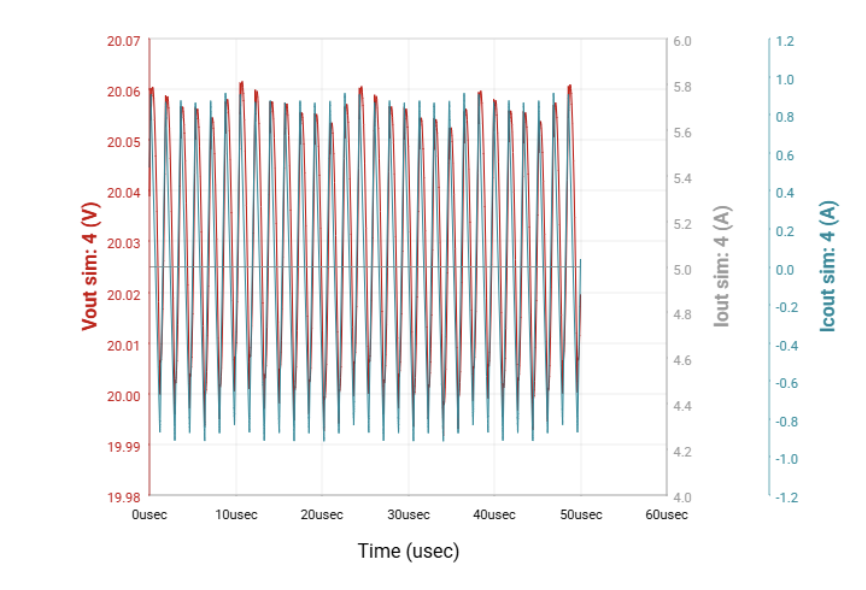
\includegraphics[width=0.8\linewidth]{images/Partie USB-C/09_Simulation de l_ondulation de la tension de sortie (Vout) et du courant capacitif (Icout) en régime permanent sous 5A.png}
    \caption{Simulation de l'ondulation de la tension de sortie (Vout) et du courant capacitif (Icout) en régime permanent sous 5A.}
\end{figure}

\textbf{Analyse~:} Cette courbe représente le comportement de notre filtre LC lorsque la carte délivre sa puissance maximale (courbe grise Iout fixée à 5~A).
\begin{itemize}
    \item \textbf{La tension de sortie (Courbe rouge / Vout)~:} On observe que la tension oscille de manière infime entre 19,99~V et 20,06~V. Cette ondulation crête-à-crête d'à peine 70~mV (soit 0,35\,\% d'erreur) est exceptionnelle.
    \item \textbf{L'action du filtre (Courbe bleue / Icout)~:} La courbe turquoise représente le courant alternatif absorbé par notre condensateur CMS de 47~$\mu$F (oscillant entre -0,9~A et +0,9~A). Elle prouve mathématiquement que le condensateur avale tout le bruit de découpage de la bobine, garantissant une tension de 20~V parfaitement lisse pour un appareil branché en USB-C.
\end{itemize}

\textbf{2. Test de choc thermique et électrique (Load Transient)}

Sur un vrai port USB-C, le courant n'est jamais constant : si l'utilisateur débranche son ordinateur chargé pour y brancher un petit écouteur, le courant chute brutalement. Il faut s'assurer que notre régulateur réagit assez vite pour ne pas créer une surtension destructrice.

\begin{figure}[H]
    \centering
    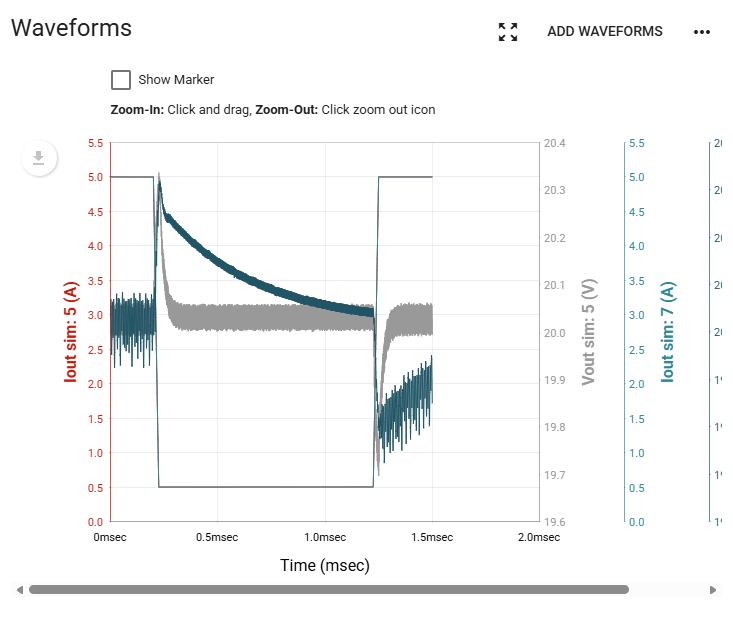
\includegraphics[width=0.8\linewidth]{images/Partie USB-C/10_Réponse de la tension (Vout) face à un changement brutal du courant demandé (Iout).png}
    \caption{Réponse de la tension (Vout) face à un changement brutal du courant demandé (Iout).}
\end{figure}

\textbf{Analyse~:}
\begin{itemize}
    \item \textbf{La contrainte (Courbe grise / Iout)~:} Nous avons simulé une variation extrême et brutale du courant, passant instantanément de la charge maximale (5~A) à une charge quasi-nulle (0,5~A), puis inversement.
    \item \textbf{La réaction du cerveau (Courbe bleue foncée / Vout)~:} Lors de la chute brutale du courant (à $t = 0,25~\text{ms}$), la tension subit un léger rebond (overshoot) bloqué à environ 20,35~V. À l'inverse, lors du fort appel de courant (à $t = 1,25~\text{ms}$), la tension chute très brièvement (undershoot) à 19,7~V avant de remonter.
\end{itemize}
\textbf{Conclusion du test~:} La tension reste toujours confinée dans une plage très sécurisée. Cela prouve que les composants de notre boucle de compensation (les résistances et condensateurs sur la broche COMP) sont parfaitement bien calculés. Le cerveau LM5116 réagit en une fraction de milliseconde pour ajuster le PWM et stabiliser la sortie.

        \subsection{Schéma détaillé et PCB}

Après avoir validé la théorie et la nomenclature industrielle, l'étape ultime a consisté à concevoir le circuit imprimé. Notre choix a été de regrouper sur une seule carte le contrôleur LM5116, la chaîne de puissance 100~W, et le convertisseur 5V/12V pour créer un module USB-C autonome.

\subsubsection*{4.1. Conception du schéma électronique (ISIS)}
Afin de faciliter la lecture, le dépannage et la future intégration avec les cartes des autres membres du groupe, le schéma ISIS a été organisé en blocs fonctionnels clairs.

\begin{figure}[H]
    \centering
    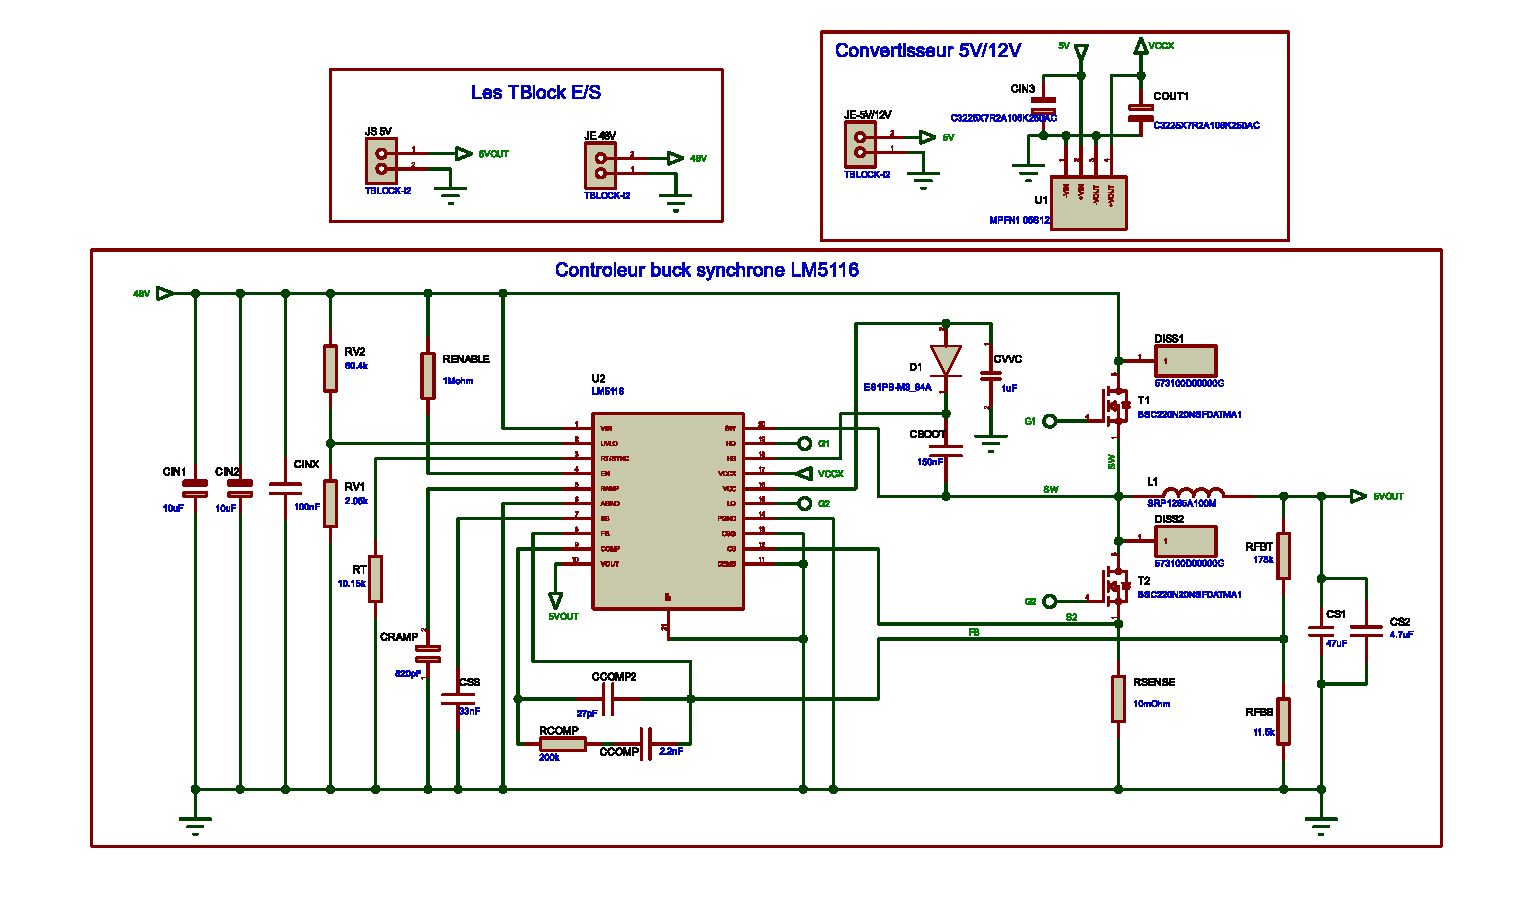
\includegraphics[width=1\linewidth]{images/Partie USB-C/11_Schéma USB-C.pdf}
    \caption{Schéma électronique complet sous Proteus.}
\end{figure}

Ce schéma comporte trois blocs distincts~:
\begin{itemize}
    \item \textbf{Les connexions E/S (TBLOCK)~:} Nous avons placé des borniers (TBLOCK) clairs pour l'entrée 48~V et pour l'alimentation 5~V externe.
    \item \textbf{Le convertisseur 5V/12V~:} Isolé en haut à droite avec ses condensateurs de filtrage, il prépare l'énergie logique pour le cerveau.
    \item \textbf{Le bloc de puissance~:} Le bloc de contrôle (LM5116), cœur du système, il intègre tous les composants passifs périphériques étudiés précédemment.
\end{itemize}

\subsubsection*{4.2. Stratégie de routage et Layout (ARES)}
Le routage final ayant été réalisé par l'encadrement technique, nous présentons ici une revue de conception pour justifier les choix stratégiques appliqués sur le circuit imprimé.

\begin{figure}[H]
    \centering
    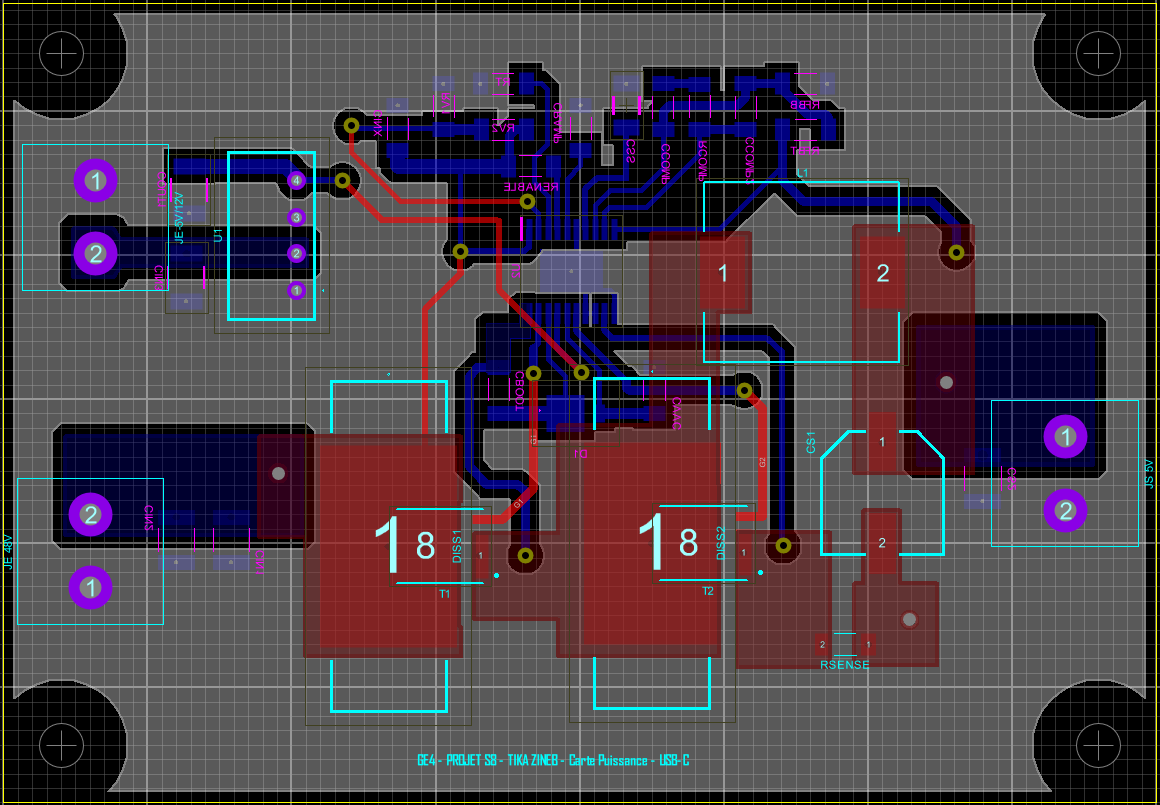
\includegraphics[width=0.8\linewidth]{images/Partie USB-C/12_PCB carte USB-C.png}
    \caption{PCB de la carte USB-C.}
\end{figure}

\begin{enumerate}
    \item \textbf{Gestion des forts courants (5A)~:} Les pistes de puissance sont dimensionnées avec une grande largeur pour éviter tout échauffement par effet Joule. Les signaux de commande restent fins.
    \item \textbf{Séparation des masses~:} La masse analogique et la masse de puissance sont physiquement séparées. Elles se rejoignent en un point unique. Cela protège le contrôleur LM5116 des parasites de commutation.
    \item \textbf{Dissipation thermique~:} L'empreinte des MOSFETs inclut de larges zones de cuivre prévues pour venir y souder nos dissipateurs thermiques CMS (DISS1 et DISS2).
    \item \textbf{Sécurité~:} Les borniers (TBLOCK) sont placés aux extrémités pour faciliter le montage final. Les indications "48V" et "5V" sur la carte évitent les inversions de polarité.
\end{enumerate}

\begin{decisionbox}[Décision : USB-C]
\textbf{Topologie :} Buck synchrone régulateur de puissance (LM5116). \\
\textbf{Pourquoi :} L'obligation d'un rendement optimal sous fort courant direct (jusqu'à $5 \, \text{A}$) nécessite une commutation synchrone pour éviter les pertes diodes. \\
\textbf{Impact système :} Intégration d'un module complexe augmentant le temps de mise au point, mais garantissant une charge stable à haute performance ($100 \, \text{W}$ max théorique) sans chauffe rédhibitoire pour l'appareil terminal.
\end{decisionbox}

    \section{USB-B}
        \subsection{Solution technique}
        L'objectif de cette section du projet est d'assurer l'alimentation du port USB-B. Le standard pour ce type d'électronique numérique étant le 5~V, nous devons abaisser la tension du bus principal industriel de 48~V vers une tension de 5~V.

        Pour répondre à ce besoin, la solution technique retenue s'articule autour d'un convertisseur DC/DC isolé 48~V/5~V. L'enjeu principal ici est double~:
        \begin{itemize}
            \item \textbf{Sécurité et isolation~:} L'isolation galvanique est primordiale pour séparer la masse de puissance (48~V) de la masse de signal (5~V). Cela protège à la fois les composants sensibles et l'utilisateur qui viendrait brancher un câble sur le port USB.
            \item \textbf{Stabilité et bruit~:} La connexion USB-B est très sensible aux parasites. Un filtre d'entrée LC a donc été mis en place pour éviter que le découpage du convertisseur ne pollue le bus 48~V.
        \end{itemize}

        \subsection{Dimensionnement des composants}
        Le choix du convertisseur a été directement dicté par les besoins de l'électronique de commande et de communication~:

        \textbf{Bilan de puissance et choix du convertisseur~:} Nous avons opté pour le module TMR\_104811WI, un convertisseur DC/DC 48/5~V isolé de 10~W. Sous 5~V, cela permet de délivrer un courant maximal de 2 ampères. Cette capacité est exactement ce que l'on veut obtenir pour notre sortie USB-B.

        \textbf{Le filtrage~:} Pour la conception de l'étage de filtrage du convertisseur, nous nous sommes appuyés rigoureusement sur le schéma de filtrage fourni par le constructeur dans la \textit{datasheet}~:

        \begin{figure}[H]
            \centering
            
\includegraphics[width=0.8\textwidth]{images/Partie USB-B/01_Schéma extrait de la datasheet.png}
            \caption{Schéma extrait de la datasheet du filtre CEM autour du convertisseur USB-B.}
        \end{figure}

        Pour la partie entrée et isolation, le choix des composants a été fait de manière à maximiser la compacité et l'efficacité face aux parasites~:

        \begin{itemize}
            \item \textbf{Filtre LC d'entrée~:} Composé d'une inductance CMS (L1) et d'un condensateur céramique de type X7R (C1). Leur rôle combiné forme un filtre qui bloque les parasites de découpage pour éviter de polluer le bus 48~V global. La très faible résistance série (ESR) du condensateur céramique lui permet de réagir instantanément aux perturbations haute fréquence.
            \item \textbf{Condensateur haute tension type Y (Isolation)~:} Placé à cheval entre la masse primaire et secondaire, ce petit condensateur de 220~pF est indispensable pour \og~court-circuiter~\fg{} le bruit de mode commun généré par le transformateur interne. Il crée un chemin de retour sécurisé, garantissant la bonne sécurité de l'USB-B.
        \end{itemize}

        \begin{tableau}[H]
            \centering
            \small
            \setlength{\tabcolsep}{4pt}
            \begin{tabular}{|l|l|p{3.8cm}|p{4.6cm}|}
                \hline
                \textbf{Composant} & \textbf{Référence} & \textbf{Caractéristiques Clés} & \textbf{Rôle} \\ \hline
                Convertisseur & TMR\_104811WI & DC/DC Isolé, 10~W, Entrée 48~V, Sortie 5~V & Abaisse le 48~V en 5~V et assure l'isolation galvanique pour protéger l'utilisateur (USB). \\ \hline
                Inductance (L1) & 74438335150 & Inductance CMS compacte (série WE-MAPI) & Associée à C1, forme un filtre d'entrée pour bloquer le bruit de découpage vers le bus 48~V. \\ \hline
                Capacité (C1) & 12101C475K4T2A & 4.7~$\mu$F, Céramique CMS (X7R), Boîtier 1210 & Découplage d'entrée~: absorbe les parasites hautes fréquences grâce à sa faible ESR. \\ \hline
                Capacité (C2) & C1812C221KGGACTU & 220~pF, Céramique Haute Tension, Boîtier 1812 & Condensateur \og~Y~\fg{}~: gère le bruit de mode commun à travers la barrière d'isolation. \\ \hline
            \end{tabular}
            \caption{Nomenclature de l'alimentation USB-B.}
        \end{tableau}

        \subsection{Schéma détaillé et PCB}
        Nous avons le schéma final suivant~:
        \begin{figure}[H]
            \centering
            \begin{subfigure}[b]{0.48\textwidth}
                \centering
                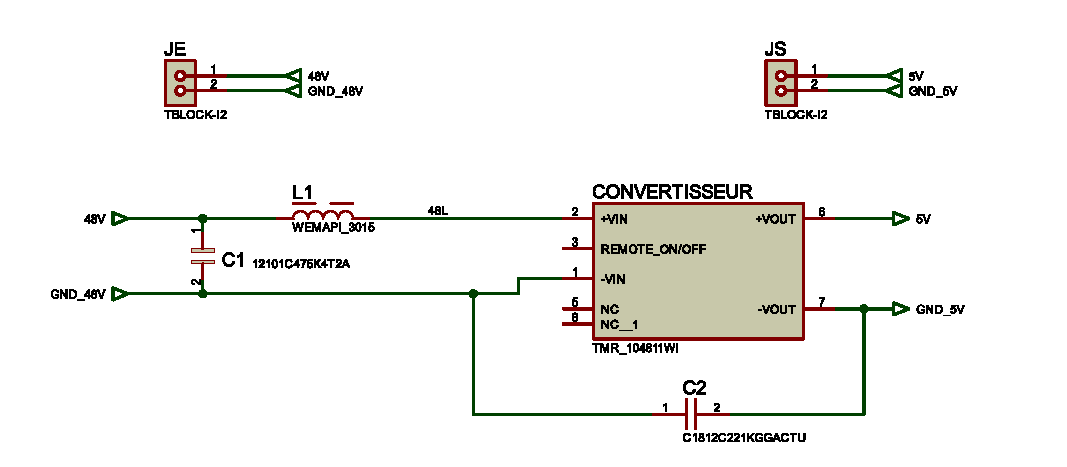
\includegraphics[width=\linewidth]{images/Partie USB-B/02_Schéma Proteus.pdf}
                \caption{Schéma du convertisseur ISO.}
            \end{subfigure}
            \hfill
            \begin{subfigure}[b]{0.48\textwidth}
                \centering
                
\includegraphics[width=\linewidth]{images/Partie USB-B/03_PCB.png}
                \caption{Routage Carte USB-B.}
            \end{subfigure}
            \caption{Conception Carte USB-B.}
        \end{figure}

\begin{decisionbox}[Décision : USB-B]
\textbf{Topologie :} Module Isolé (TMR 104811WI) $48 \, \text{V} \to 5 \, \text{V}$ / $10 \, \text{W}$. \\
\textbf{Pourquoi :} Assurer l'isolation galvanique entre le bus industriel haute puissance ($48 \, \text{V}$) et l'utilisateur, limitant les risques électriques en cas de défaut. \\
\textbf{Impact système :} Sécurisation totale du port de charge classique au prix d'un encombrement matériel et un rendement global très légèrement inférieur aux solutions non isolées.
\end{decisionbox}

    \section{Alimentation de la logique de commande}
        \subsection{Solution technique}
        L'objectif de cette section du projet est d'assurer l'alimentation de l'ensemble de la logique de commande (microcontrôleurs PIC) ainsi que des \textit{drivers} destinés à d'autres cartes périphériques. L'électronique numérique standard fonctionnant en 5~V, nous devons abaisser la tension du bus principal industriel de 48~V vers une tension de 5~V.

        Pour répondre à ce besoin, la solution technique retenue s'articule autour du convertisseur DC/DC isolé BCT40T48S05. Ce choix de composant repose sur ses caractéristiques industrielles de haute performance~: il est capable de délivrer une puissance de 40~W, ce qui représente un courant maximal de 8 ampères sous 5~V.

        Bien que la consommation théorique cumulée de nos microcontrôleurs et de nos \textit{drivers} soit inférieure à cette limite, ce surdimensionnement volontaire est une décision stratégique de conception. Il présente trois avantages majeurs~:
        \begin{itemize}
            \item \textbf{Fiabilité thermique~:} Le convertisseur ne fonctionnant jamais à sa limite maximale, il dissipera beaucoup moins de chaleur, prolongeant ainsi sa durée de vie.
            \item \textbf{Stabilité~:} Il encaissera sans aucune chute de tension les appels de courant brusques générés par l'activation simultanée de plusieurs \textit{drivers}.
            \item \textbf{Évolutivité~:} Cette réserve de puissance permettra d'alimenter d'éventuelles cartes supplémentaires à l'avenir sans devoir repenser l'alimentation.
        \end{itemize}

        Pour accompagner cette forte puissance, un réseau de filtrage d'entrée robuste a été mis en place pour éviter que le convertisseur ne pollue le bus 48~V, tandis que le filtrage de sortie a fait l'objet d'une stratégie de décentralisation (au plus près des puces) pour s'adapter aux forts courants distribués.

        \subsection{Dimensionnement des composants}
        Le choix du convertisseur a été directement dicté par les besoins énergétiques cumulés de la logique et des \textit{drivers} de puissance~:

        \textbf{Bilan de puissance et choix du convertisseur~:} Notre système devant distribuer du 5~V à plusieurs cartes, nous avons opté pour le module BCT40T48S05. Il s'agit d'un convertisseur DC/DC isolé de 40~W. Sous 5~V, cela permet de délivrer un courant total allant jusqu'à 8 ampères. Cette forte capacité nous assure de pouvoir alimenter tous les PICs et les \textit{drivers} sans aucune chute de tension, tout en conservant une excellente marge de sécurité thermique.

        \textbf{Le filtrage~:} Pour la conception de l'étage de filtrage du convertisseur, nous nous sommes appuyés rigoureusement sur le schéma d'application d'un convertisseur de même type que celui choisi avec en sortie une charge~:

        \begin{figure}[H]
            \centering
            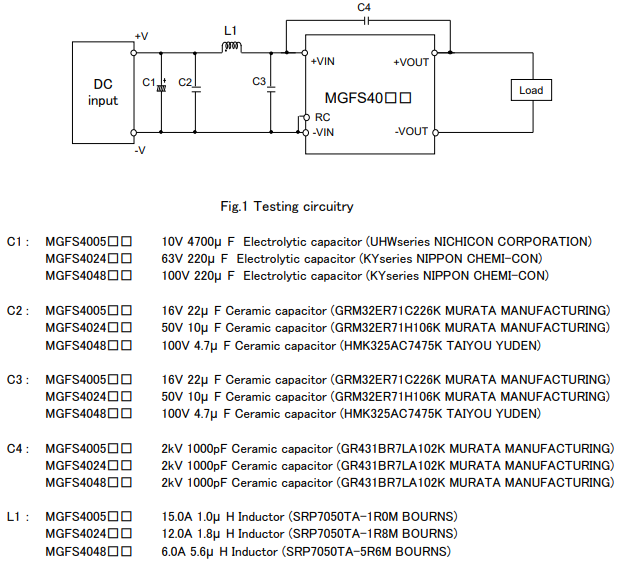
\includegraphics[width=0.8\textwidth]{images/Partie Filtre ALIM/01_Schéma extrait de la datasheet.png}
            \caption{Schéma extrait de la datasheet du filtre CEM autour du convertisseur 40~W.}
        \end{figure}

        Pour la partie entrée et isolation, le choix des composants a été fait pour maximiser l'immunité aux bruits de découpage~:

        \begin{itemize}
            \item \textbf{Condensateur électrolytique (C1)~:} Placé en tête de ligne (100~$\mu$F), il agit comme un gros réservoir d'énergie pour absorber les appels de courant globaux lorsque les \textit{drivers} s'activent.
            \item \textbf{Filtre en entrée (C2, L2, C3)~:} L'association d'une inductance et de deux condensateurs céramiques CMS de 4.7~$\mu$F (technologie X7R) forme un filtre passe-bas bidirectionnel très performant. Grâce à leur très faible résistance série (ESR), les condensateurs réagissent instantanément pour bloquer les parasites haute fréquence et éviter qu'ils ne remontent polluer le bus 48~V.
            \item \textbf{Condensateur haute tension type Y (C4)~:} Placé à cheval entre la masse primaire et secondaire, ce condensateur de 1000~pF est indispensable pour \og~court-circuiter~\fg{} le bruit de mode commun généré par le transformateur interne du convertisseur, maintenant ainsi un 5~V très propre.
        \end{itemize}

        \begin{tableau}[H]
            \centering
            \footnotesize
            \setlength{\tabcolsep}{4pt}
            \begin{tabular}{|l|l|p{3.8cm}|p{4.6cm}|}
                \hline
                \textbf{Composant} & \textbf{Référence} & \textbf{Caractéristiques Clés} & \textbf{Rôle} \\ \hline
                Convertisseur & BCT40T48S05 & DC/DC Isolé, 40~W, Entrée 48~V, Sortie 5~V & Abaisse le 48~V en 5~V. Fournit jusqu'à 8~A pour alimenter l'ensemble de la logique et des \textit{drivers}. \\ \hline
                Inductance (L) & B82462G4472M000 & 4,7~$\mu$H Inductance CMS de puissance & Associée à C4 et C2, forme un filtre LC d'entrée. \\ \hline
                Capacité (C1) & 72SXE100M+T & 100~$\mu$F Électrolytique, forte capacité & Réservoir d'énergie global pour l'entrée. \\ \hline
                Capacités (C2, C3) & GRM31CZ72A475KE11L & 4.7~$\mu$F, Céramique CMS (X7R) & Découplage d'entrée (Filtre LC)~: absorbe les parasites HF grâce à sa faible ESR. \\ \hline
                Capacité (C4) & CC1812JKNPODBN102 & 1000~pF Céramique Haute Tension & Condensateur \og~Y~\fg{}~: gère le bruit de mode commun à travers la barrière d'isolation. \\ \hline
            \end{tabular}
            \caption{Nomenclature de l'alimentation PIC.}
        \end{tableau}

        \subsection{Schéma détaillé et PCB}
        Nous avons le schéma final suivant~:
        \begin{figure}[H]
            \centering
            \begin{subfigure}[b]{0.48\textwidth}
                \centering
                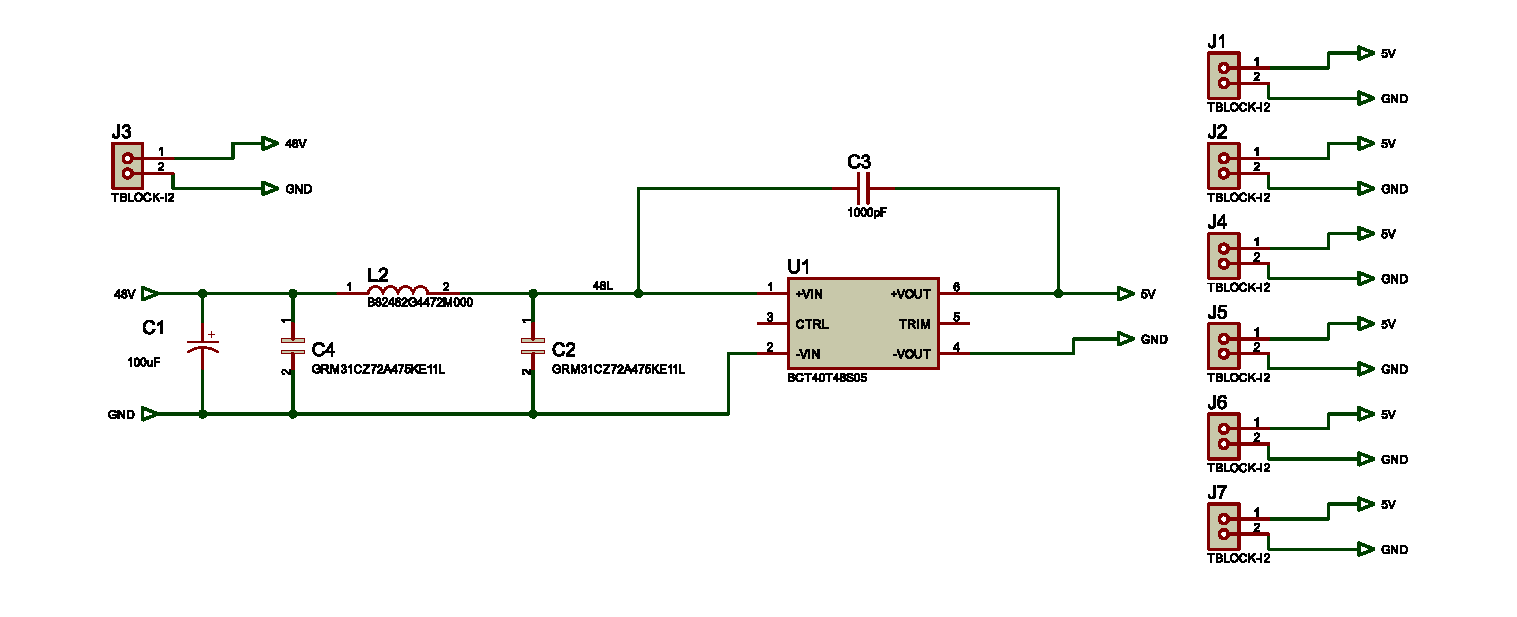
\includegraphics[width=\linewidth]{images/Partie Filtre ALIM/02_Schema Proteus.pdf}
                \caption{Schéma du filtre 40 W.}
            \end{subfigure}
            \hfill
            \begin{subfigure}[b]{0.48\textwidth}
                \centering
                
\includegraphics[width=\linewidth]{images/Partie Filtre ALIM/03_PCB.png}
                \caption{Routage de la carte.}
            \end{subfigure}
            \caption{Conception Alimentation Logique.}
        \end{figure}

\begin{decisionbox}[Décision : Alimentation Logique]
\textbf{Topologie :} Module DC/DC isolé fort courant BCT40T48S05 ($48 \to 5 \, \text{V}$ / $40 \, \text{W}$). \\
\textbf{Pourquoi :} Le dimensionnement à $8 \, \text{A}$ garantit que la logique (Microcontrôleurs, bus CAN) ne subira aucune variation (brownout) lors des transitoires d'activations de relais/drivers. \\
\textbf{Impact système :} Suppression des bugs aléatoires de reset CPU, fiabilité accrue du bus CAN et immunité galvanique vis-à-vis des étages de puissance.
\end{decisionbox}

